\documentclass[anon,12pt]{alt2025} % Anonymized submission
%\documentclass[final,12pt]{alt2025} % Include author names


%%% Our includes
\usepackage{amsmath}
\usepackage[capitalise,noabbrev]{cleveref}
\usepackage{graphicx}
\usepackage{mdframed}
\usepackage{paralist}
\usepackage{wrapfig}
\usepackage{dsfont}
\usepackage{thmtools}
\usepackage{thm-restate}
\usepackage{xfrac}


%%% Our new defines
\newcommand{\vect}[1]{\ensuremath {\mathbf{#1}}}
\newtheorem{claim}{Claim}


\title[Online Non-Linear Covering with Multiple Experts]{Online Non-Linear Covering with Multiple Experts}
\usepackage{times}
% Use \Name{Author Name} to specify the name.
% If the surname contains spaces, enclose the surname
% in braces, e.g. \Name{John {Smith Jones}} similarly
% if the name has a "von" part, e.g \Name{Jane {de Winter}}.
% If the first letter in the forenames is a diacritic
% enclose the diacritic in braces, e.g. \Name{{\'E}louise Smith}

% Two authors with the same address
% \altauthor{\Name{Author Name1} \Email{abc@sample.com}\and
%  \Name{Author Name2} \Email{xyz@sample.com}\\
%  \addr Address}

% Three or more authors with the same address:
% \altauthor{\Name{Author Name1} \Email{an1@sample.com}\\
%  \Name{Author Name2} \Email{an2@sample.com}\\
%  \Name{Author Name3} \Email{an3@sample.com}\\
%  \addr Address}

% Authors with different addresses:
\altauthor{%
 \Name{Eniko Kevi} \Email{eniko.kevi@univ-grenoble-alpes.fr}\\
 \Name{Nguyen Kim Thang} \Email{kim-thang.nguyen@univ-grenoble-alpes.fr}\\
 \addr 150 Pl. du Torrent, 38400 Saint-Martin-d'Heres, France
}

\begin{document}
\maketitle

\begin{abstract}
    Auctions with divisible resources represent various practically relevant problems, such as network bandwidth allocation and food aid distribution. In each of these settings, the desire to receive (or the need of) a resource is represented by bids. The proportional allocation mechanism assigns a fraction of the resource to each bidder in proportion to the bid across all the bids. Despite the importance of these type of auctions, the efficiency of proportional allocations is still not completely understood. In recent years, \cite{Tardos2013} proved a lower bound of $26.8\%$ for the Price of Anarchy (PoA) considering social welfare, and \cite{Caragiannis2014} improved their analysis to $50\%$ both for social and effective welfares. This paper follows a different perspective on the analysis of this problem, which relies on the primal-dual method (first introduced in this setting by \cite{Thang2017}). We prove that the Price of Anarchy (PoA) bound considering the effective welfare of proportional allocation over coarse-correlated and Bayes-Nash equilibria in the complete information setting for a single item is $50\%$, and this result is \emph{tight}.
\end{abstract}

\begin{keywords}
    learning-augmented algorithm, non-linear objective, multiple experts, multiple oracles, primal-dual algorithm, covering problem, predictions, online algorithm with advice
\end{keywords}

%!TEX root = ./main.tex

\section{Introduction}

% Introduction and motivation for our problem
% main objective: compare the best combination of experts.
% So for in the literature, always compare to the best expert (ex., regret)

The domain of algorithms with predictions \cite{MitzenmacherVassilvitskii20:Beyond-the-Worst-Case}  (or learning-augmented algorithms) emerged recently and grew immensely at the intersection of (discrete) algorithm design and machine learning (ML).
Combining ML techniques with traditional algorithm design methods enables online algorithms to benefit from predictions that can infer future information from patterns in past data. Online algorithms with predictions can obtain performance guarantees beyond the worst-case analysis and provide fine-tuned solutions to various problems. In the literature, many significant problems have new learning-augmented results, for example, scheduling \cite{LattanziLavastida20:Online-scheduling,Mitzenmacher20:Scheduling-with}, caching (paging) \cite{LykourisVassilvtiskii18:Competitive-caching,Rohatgi20:Near-optimal-bounds,AntoniadisCoester20:Online-metric}, ski rental \cite{GollapudiPanigrahi19:Online-algorithms,KumarPurohit18:Improving-online,AngelopoulosDurr20:Online-Computation}, counting sketches \cite{HsuIndyk19:Learning-Based-Frequency}, bloom filters \cite{KraskaBeutel18:The-case-for-learned,Mitzenmacher18:A-model-for-learned}, and metrical task systems \cite{AntoniosEtAll23:mixing-predictions-metric-algorithms}.

Even though predictions provide a glimpse of the future, there is no mathematical guarantee for their accuracy. Adjusting the algorithm's trust in the predictions is a significant challenge since online algorithms must make irrevocable decisions at each time step. Ideally, if the predictions are accurate, the algorithm should perform well compared to the offline setting. In contrast, if the predictions are misleading, the algorithm should maintain a competitive solution, similar to the online setting where no predictive information is available. In other words, online algorithms with predictions are expected to bring the best of both worlds: mathematical performance guarantees of classical algorithms and good future prediction capabilities of machine learning methods.

Predictions can come from multiple sources (for example: heuristics, oracles, and randomized methods), but we ignore their nature and call all of them \emph{experts}.  An algorithm's consistency with the experts' suggestions is typically measured by comparing the algorithm's result with the solution of the \emph{best} expert. A representative example is the popular notion of regret in online learning, which fueled the development of many powerful algorithms and techniques.

A natural research question is whether it is possible to design competitive algorithms with mathematical performance guarantees with a stronger benchmark than the best expert. Comparing an algorithm with a stronger benchmark could provide deeper insights into the learning process and give better ways of exploiting the experts' predictions.

Taking a broader view, we can study whether combining predictions of several experts is similar to combining multiple online algorithms and whether we can expect to achieve better solutions with the combination. Assuming that we do not know in advance which of the given algorithms would perform best on the upcoming requests, can we combine the algorithms in some generic way to obtain a competitive online strategy? This has been a long-standing question in the community of online algorithms \cite{AzarBroder93:On-line-Choice,BlumBurch00:On-line-Learning}. To find an answer, it is a crucial to understand to what extent such an online strategy can benefit from the input of multiple algorithms and what is a suitable benchmark to evaluate its performance.

While in a completely general setting such an online strategy and a corresponding benchmark may not exist, in this paper we propose
two algorithms for online linear and convex problems with covering constraints that are competitive with the new benchmark (informally the \emph{best linear combination} of the experts). Therefore, our paper partially addresses the question we raised in the previous paragraph.

\subsection{Model and Problem}

\paragraph{Covering problem with experts.}
In the linear problem setting, we have $n$ resources and each resource $i$ has a cost per unit $c_{i}$ that we know in advance ($1 \leq i \leq n$).
Let $x_{i}$ be a non-negative variable representing the amount chosen from resource $i$.
The total cost of a solution $(x_{i})_{i=1}^{n}$ is $\sum_{i=1}^{n} c_{i} x_{i}$.
The problem includes $K$ experts and the problem's covering-type constraints are revealed online one-by-one.
At each time $t \geq 1$, we receive a covering constraint $\sum_{i=1}^{n} a_{i}^{t} x_{i} \geq 1$ (where $a_{i}^{t} \geq 0$) and each expert $k$ (where $1 \leq k \leq K$) provides
a solution $(s_{i,k}^{t})_{i=1}^{n}$. Our algorithm can observe the experts' solutions and afterwards it must update its own solution (denoted as $(x_{i}^{t})_{i=1}^{n}$)
to satisfy the new constraint, while maintaining the satisfaction of the previous ones. This algorithm must update its solution in the sense of online algorithms, so it cannot modify the previously made decisions. Formally, $x_{i}^{t} \geq x_{i}^{t-1} ~\forall\ i, t$.
Our goal is to design an algorithm that minimizes $\sum_{i=1}^{n} c_{i} x_{i}^{T}$ subject to
all online covering constraints $t$, where $1 \leq t \leq T$. The value $T$ is the last time a constraint is released, and it is not known by the algorithm.

The convex problem setting is analogous to the linear one, since we consider convex problems with linear constraints. The only difference compared to the previous paragraph is the total cost of the solution $(x_{i})_{i=1}^{n}$, which becomes $f(x)$, where $f$ is a convex function.

\paragraph{Experts.} \label{subsec:experts} In our model, the experts' predictions are also online solutions. In other words, the experts' solutions
fulfill the following properties:
\begin{enumerate}
	\item for every expert $k$ and for every time $t$ the solution $(s_{i,k}^{t})_{i=1}^{n}$ is feasible, therefore, every constraint $t'$ where $1 \leq t' \leq t$ is satisfied;
	\item for every expert $k$ and for every time $t$ and for every resource $i$, the previous expert solutions are irrevocable, therefore $s_{i,k}^{t} \geq s_{i,k}^{t'}$ for all $t' \leq t$.
\end{enumerate}
These properties can be verified online. If some experts do not satisfy them, we simply ignore those experts both in the decision-making and in the benchmark.
A crucial remark: we do \emph{not} assume that the experts' solutions are tight at each constraint $t$, requiring $\sum_{i=1}^{n} a_{i}^{t} s_{i,k}^{t} = 1 ~ \forall t, k$ to hold.
This assumption is unrealistic and cannot be maintained in an online manner (see the discussion in Appendix~\ref{appix-tight-solutions}).
Besides, assuming tight constraint satisfaction would simplify the problem, while intuitively,
the difficulty of designing competitive algorithms comes from the lack of obvious ways to distinguish
good expert solutions from (probably many) non-efficient/misleading ones.

\paragraph{Benchmark.}
We consider a dynamic benchmark that captures the \emph{best linear combination} of all experts' solutions \emph{over time}.
Informally, at any online time step, the benchmark can take a linear combination of the experts' solutions.
The linear combination can be changed over time, and it can be different from previous combinations.
However, the benchmark's decisions are also online, so it cannot decrease the value of the decision variables ($x_{i}$).
We refer to our benchmark with the name \texttt{LIN-COMB} from now on.

The \texttt{LIN-COMB} benchmark's formal description is visible on \cref{fig:benchmark}.
Let $w_{k}^{t} \geq 0$ be the weight assigned by the \texttt{LIN-COMB} benchmark to expert $k$ (where $1 \leq k \leq K$) at time~$t$.
Since we consider a linear combination, the constraint $ \sum_{k=1}^{K} w_{k}^{t} = 1$ must hold.
%In the linear program, we consider the relaxed version of this constraint, where $\sum_{k=1}^{K} w_{k}^{t} \geq 1$.
The solution of \texttt{LIN-COMB} at time $t$ is ideally $x_{i}^{t} = \sum_{k=1}^{K} w_{k}^{t} s_{i,k}^{t}$,
however, $x_{i}^{t}$ must be larger than $x_{i}^{t-1}$.
Therefore, we set $x_{i}^{t} = \max\bigl\{\sum_{k=1}^{K} w_{k}^{t} s_{i,k}^{t},\ x_{i}^{t-1}\bigr\}$.
In other words, given the chosen weights, if  $\sum_{k=1}^{K} w_{k}^{t} s_{i,k}^{t} < x_{i}^{t-1}$ then $x_{i}^{t} \gets x_{i}^{t-1}$,
otherwise $x_{i}^{t} \gets \sum_{k=1}^{K} w_{k}^{t} s_{i,k}^{t}$.

\begin{figure}[ht]
	\begin{mdframed}
	%	\begin{spacing}{0.1}
		\begin{align*}
			\text{Linear objective:} && \min \sum_{i=1}^{n} c_{i} x_{i}^{T} &= \min \sum_{i=1}^{n} c_{i} \sum_{t=1}^{T}\bigl( x_{i}^{t} - x_{i}^{t-1}\bigr)\\
			\text{Convex objective:} && \min f(x^{T}) &\\
	%	\end{align*}
	%	subject to
	%	\end{spacing}
	%	\begin{align*}
		&& & \\
		\text{Subject to (in both cases):} &&
			\sum_{k=1}^{K} w_{k}^{t} &= 1  && \forall\ t \\
			%
			&& x_{i}^{t} &\geq \sum_{k=1}^{K} w_{k}^{t} s_{i,k}^{t} && \forall\ i, t\\
			%
			&& x_{i}^{t} &\geq x_{i}^{t-1} && \forall\ i, t\\
			%
			&& w_{k}^{t} &\geq 0  && \forall\ t, k
		\end{align*}
		where $1 \leq t \leq T$, $1 \leq i \leq n$, and $f$ is convex.
		\vspace{5pt}
	\end{mdframed}
	\caption{Formulation of the \texttt{LIN-COMB} benchmark for both the linear and convex problems}
	\label{fig:benchmark}
	\end{figure}

Since every expert's solution is feasible by our assumptions, at each time $t$ and for all resource $i$ (where $1 \leq i \leq n$),
the constructed solution $x_{i}^{t} \geq \sum_{k=1}^{K} w_{k}^{t} s_{i,k}^{t}$ constitutes a feasible solution to the covering constraints of the original covering problem.
Formally, for every constraint $t'$ with $t' \leq t$,
%
\begin{align*}
\sum_{i=1}^{n} a_{i}^{t'} x_{i}^{t} \geq
%
\sum_{i=1}^{n} a_{i}^{t'} \biggl( \sum_{k=1}^{K} w_{k}^{t} s_{i,k}^{t} \biggr)
%
	= \sum_{k=1}^{K} w_{k}^{t}  \biggl( \sum_{i=1}^{n} a_{i}^{t'} s_{i,k}^{t} \biggr)
%
	\geq \sum_{k=1}^{K} w_{k}^{t} \geq 1
\end{align*}
%
where the second inequality holds due to the feasibility of the experts' solutions.
%
%Let $y_{i}^{t}$ be a variable representing the increase of $x_{i}^{t}$ compared to $x_{i}^{t-1}$. The benchmark is as follows.
%%
%\begin{align*}
%    && \min \sum_{t = 1}^{T} \sum_{i=1}^{n} & c_i y_i^t \\
%%
%    (\alpha^{t}) \qquad && \sum_{k=1}^{K} w_{k}^{t} & \geq 1  & \forall\ 1 \leq t \leq T,\ 1 \leq i \leq n \\
%%
%    (\beta_{i}^{t}) \qquad && \sum_{k=1}^{K} \left(w_{k}^{t} s_{i,k}^{t} - w_{k}^{t-1} s_{i,k}^{t-1} \right) &\leq y_i^t  &\forall\ 1 \leq t \leq T,\ 1 \leq i \leq n\\
%%
%    && w_{k}^{t},\ y_{i}^{t} & \ge 0 & \forall\ 1 \leq t \leq T,\ 1 \leq i \leq n,\ 1 \leq k \leq K
%\end{align*}
%
We highlight that the best-expert benchmark is included in \texttt{LIN-COMB}. We get the solution of this benchmark by setting $w^{t}_{k^{*}} = 1$ for all $t$, where $1 \leq t \leq T$, and $w^{t}_{k} = 0$ for all $k \neq k^{*}$,
where $k^{*}$ is the best expert (so $x_{i}^{t} = s_{i,k^{*}}^{t}$ for all $i$ and $t$).

\subsection{Our approach and contribution}

\paragraph{Approach.} We use the primal-dual approach to design competitive algorithms with the new \texttt{LIN-COMB} benchmark. First, we relax the linear program formulation of \texttt{LIN-COMB}, which serves as a lower bound. Then, we take the dual of the relaxation, which is a lower bound on the relaxation. Therefore, following the chain of lower bounds, the dual problem is a lower bound on the \texttt{LIN-COMB} benchmark. The formulations of the relaxation and its dual is detailed in \cref{sec:covering} for linear problems and in \cref{sec:convex} for convex problems.

Both of our proposed algorithms set the decision variables at every time step based on the solution of an internal convex program. Our approach is inspired by the
convex regularization method of \cite{BuchbinderChen14:Competitive-Analysis}, where the objective of the convex program is a shifted entropy function.
These functions have been widely used, in particular in the recent breakthrough related to $k$-server \cite{BubeckCohen18:K-server-via-multiscale,BuchbinderGupta19:k-servers-with}
and metrical task system problems \cite{BubeckCohen21:Metrical-task},
in which the entropy functions are shifted by constant parameters.

\paragraph{Novelty.} A novel point in our approach is that the entropy function is shifted by the average of the experts' solutions.
Moreover, regarding the constraints of the convex program, instead of using the experts' solutions directly,
we define auxiliary solutions that guarantee tight constraint satisfaction. We only use these tight solutions in the constraints and they play a crucial role in the proofs.

\paragraph{Results.} Let $\rho$ be the maximum ratio between the experts' solutions on the resources. Formally,
%We define the following parameter to establish the competitive ratio of our algorithm.
\[
	\rho := \max_{i} \max_{t',t''} \biggl\{\frac{\sum_{k=1}^{K} s_{i,k}^{t'}}{\sum_{k=1}^{K} s_{i,k}^{t''}} \biggr\}  \textnormal{ s.t. } \sum_{k=1}^{K} s_{i,k}^{t''} > 0.
\]
Informally, $\rho$ represents the discrepancy across the experts' predictions.
Our main result consists of two algorithms. The first one (which provides solutions for online linear covering) has an objective cost at most $O(\ln(K\rho))$ times the cost of the \texttt{LIN-COMB} benchmark. The second one (for online convex covering) achieves an objective cost at most $O(\ln(K\rho)) \cdot \frac{\lambda}{(1-\mu\ln(K\rho))}$ times the cost of \texttt{LIN-COMB}, where $\lambda$ and $\mu$ are the ($\lambda$,$\mu$)-smoothness parameters of the objective function.
In particular, for $0$-$1$ optimization problems, where the experts provide integer (deterministic or randomized) solutions, our first algorithm is $O(\ln(K))$-competitive with \texttt{LIN-COMB}, and the second one is $O(\ln(K)) \cdot \frac{\lambda}{(1-\mu\ln(K))}$-competitive.
An interesting feature of our algorithms is their resilience to the fluctuation of the quality of predictions (discussed in \cref{subsec:related-works} and illustrated with experiments in \cref{sec:exp}).

\subsection{Related work and discussions} \label{subsec:related-works}

Much of the research focusing on surpassing worst-case performance guarantees is motivated by the spectacular advances of machine learning (ML). Specifically, ML methods can detect patterns among the arriving input requests and provide valuable insights for the online algorithms regarding future requests. \cite{LykourisVassilvtiskii18:Competitive-caching} introduced a general framework to integrate ML predictions into classical algorithm designs to surpass the worst-case performance limit.
As a result, many practically relevant online problems were revisited to enhance existing classical algorithms with ML predictions (see the aforementioned \cite{LattanziLavastida20:Online-scheduling,Mitzenmacher20:Scheduling-with,LykourisVassilvtiskii18:Competitive-caching,Rohatgi20:Near-optimal-bounds,AntoniadisCoester20:Online-metric,GollapudiPanigrahi19:Online-algorithms,KumarPurohit18:Improving-online,AngelopoulosDurr20:Online-Computation,HsuIndyk19:Learning-Based-Frequency,KraskaBeutel18:The-case-for-learned,Mitzenmacher18:A-model-for-learned,AntoniosEtAll23:mixing-predictions-metric-algorithms}).

On a high-level view, we aim to design algorithms that are robust (competitive) to the offline optimal solution and also consistent with the expert's predictions. Ideally, the performance of the designed algorithm should surpass previous bounds whenever the predictions are reliable (low errors).
However, most learning-augmented algorithms suffer when the error rates are neither very low nor very high, resulting in prediction confidence that is neither very low nor very high.
Figure~\ref{fig:robustness-consistency} provides a general picture of the performance of an algorithm with predictions, which is representative for many problems (for example, \cite{BamasMaggoriSvensson20:primal-dual-method,KeviNguyen23:Primal-Dual-Algorithms}).

\begin{wrapfigure}{r}{0.4\textwidth}
	\vspace{-1.2cm}
	\begin{center}
		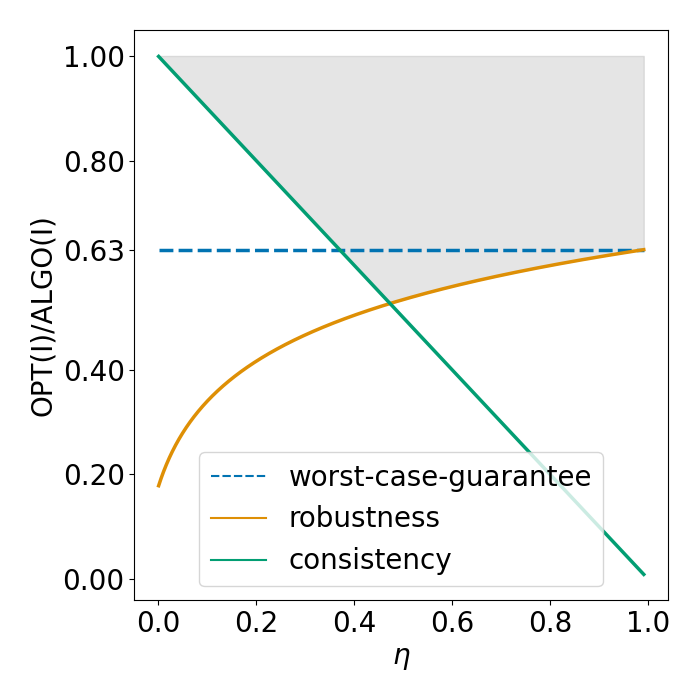
\includegraphics[width=0.4\textwidth]{../paper/Img/consistency_robustness.png}
	\end{center}
	\vspace{-1cm}
	\caption{Robustness-Consistency}
	\label{fig:robustness-consistency}
	\vspace{-0.2cm}
\end{wrapfigure}

\noindent In the figure, $\eta$ indicates the confidence in the predictions (or equivalently the error rate of predictions). The learning-augmented algorithm's performance bound is the maximum value of the green and orange curves (gray shaded area on the figure). We can observe that when $0.4 \leq \eta \leq 0.9$,
the algorithm's performance guarantee is worse than the classical worst-case guarantee (that can be achieved by simply ignoring all predictions).
Intuitively, in the case of neither very low nor very high confidence in the predictions, the algorithm has a hard time deciding if it should follow the predictions or the best-known standard algorithm in the worst-case paradigm.
It naturally raises the question whether we can achieve at least a constant factor of the worst-case guarantee (where the constant is as close to 1 as possible), while assuring a resilient output solution regardless of the predictions' quality.
Our algorithms with the new benchmark provides an answer to this question.


The paper of \cite{AnandGe22:Online-Algorithms} is the closest to ours, which also studies the design of algorithms with multiple experts.
They consider a \texttt{DYNAMIC} benchmark that is intuitively
the minimum cost solution that is supported by at least one expert solution at each time step. Formally:
\[\texttt{DYNAMIC} = \min_{\hat{\textbf{x}} \in \hat{X}} \sum_{i=1}^{n} c_i \hat{x}_i \textnormal{, where}\]
%
\[\hat{X} = \{\hat{\vect{x}} : \forall\ i \in [n],\ \forall\ t \in [T],\ \exists\ k \in [K]\ \textnormal{ such that } s_{i,k}^{t} \le \hat{x}_i \}\]
%
Our benchmark, \texttt{LIN-COMB}, is included in \texttt{DYNAMIC}, since every solution $x_{i}^{t}$ in \texttt{LIN-COMB} satisfies:
\[
	x_{i}^{t} \geq \sum_{k} s_{i,k}^{t}w_{k}^{t} \geq \min_{k} \{s_{i,k}^{t}\}
\]
therefore, for any $i$ and $t$, there exists $k$ such that $x_{i}^{t} \geq s_{i,k}^{t}$.
However, the inverse is not true: a solution $\hat{\vect{x}}^{t} \in \hat{X}$ in \texttt{DYNAMIC} is not necessarily
a linear combination of the experts' solutions.
The \texttt{DYNAMIC} benchmark in \cite{AnandGe22:Online-Algorithms} relied on the assumption that at every time step
the experts' solutions are tight. This assumption does not allow the representation of some realistic problems and it is impossible to maintain in online solutions (see Appendix~\ref{appix-tight-solutions}).
Further, \cite{AnandGe22:Online-Algorithms} claimed an $O(\ln(K))$-competitive algorithm in the \texttt{DYNAMIC} benchmark.
Unfortunately, their benchmark is too strong; we show an example in Appendix~\ref{sec:counter-example}
in which their algorithm's performance guarantee is unbounded in their \texttt{DYNAMIC}
benchmark. We believe that with a different benchmark their algorithm could be $O(\ln(K))$-competitive, however, we did not manage to prove this.


Integrating multiple predictions into online algorithms was a topic of other papers as well.
As an example, \cite{GollapudiPanigrahi19:skirental-multiple-predictions} studied the ski rental problem with multiple predictions.
The authors defined a consistency metric, which compares the performance of their algorithm to the optimal solution, given that at least one prediction (among the $k$ predictions) is optimal.
%By carefully integrating every prediction in their algorithm design, the authors managed to reduce the overall prediction error rate and obtain the best possible performance guarantee for their algorithm. During their analysis, they defined a consistency metric, which compares the performance of their algorithm to the optimal solution, given that at least one prediction (among the $k$ predictions) is correct.
\cite{AlmanzaChierichetti21:Online-Facility} also considered multiple predictions in the online facility location problem.
%The suggestions are treated as a family of sets and the authors use the union of these suggestions.
They compared the performance of their algorithm to the best possible solution obtained on the union of the suggestions. Recently, \cite{DinitzIm:Algorithms-with} studied the use of multiple predictors for several problems such as matching, load balancing, and non-clairvoyant scheduling. They provided algorithms competitive to the best predictor for such problems.
An important remark: all the above benchmarks are captured within \texttt{LIN-COMB}.

Furthermore, \cite{AntoniosEtAll23:mixing-predictions-metric-algorithms} proposed an algorithm with multiple experts for the metrical task system problem. Their benchmark allows switching from one expert to another at each time step, but it does not allow combinations of experts or any solution not suggested by one of the experts. In our \texttt{LIN-COMB} benchmark, the linear combinations that evolve over time could result in a solution that is not suggested by one of the experts and potentially, they can be much more efficient. In \cite{AntoniosEtAll23:mixing-predictions-metric-algorithms} there is a cost for state transitions, which is appropriate for their problems, but in many other problems, the smooth transition with additional costs from previous decisions to new ones is not allowed (past decisions are immutable). Therefore, the results of \cite{AntoniosEtAll23:mixing-predictions-metric-algorithms} are not applicable to our setting.

Combining online algorithms into a new algorithm to achieve better results than the individual input algorithms has been a long-standing online algorithm design question \cite{AzarBroder93:On-line-Choice,BlumBurch00:On-line-Learning}.
Its intrinsic difficulty is similar to the issue we mentioned earlier: when the performance of the given input algorithms (or heuristics) is unclear (especially in the online setting), it is challenging to create a combination that can surpass the performance of the included algorithms.
Following the current development of online algorithm design techniques with multiple predictions, this subject has been renewed with different machine learning approaches. Our paper contributes to this line of research.

\subsection{Paper overview}

In this paper we show two algorithms to solve online \emph{linear} and online \emph{convex} covering problems with multiple experts. While the convex setting includes the linear one, our proposed algorithm is simpler for the linear case. Therefore, \cref{sec:covering} details our first algorithm for the linear case, and afterwards, in \cref{sec:convex} we detail the extension to the convex case. \cref{sec:exp} shows empirical results, and we conclude in \cref{sec:conclusion}.
%!TEX root = ./main.tex

\section{The framework}		\label{sec:covering}

\subsection{Formulation}
We formulate the online covering problem that we described in the Preliminaries as a problem of finding the minimum cost solution among all the possible solutions. This formulation has an exponential number of variables and constraints; however, it allows us to transform the non-linear objective function into a linear one, which is crucial for our algorithm and proofs.

Let $S \subseteq \mathcal{E}$ be a \emph{solution} if $\one_{S}$ corresponds to a feasible solution. Let $x_{e}$ be a variable indicating whether resource $e$ is selected.
Let $z_{S}$ be an indicator variable for solution $S$. If $z_{S} = 1$, then every variable
$x_{e} = 1$ if $e \in S$, and $x_{e} = 0$ if $e \notin S$. Otherwise, $z_S = 0$. In other words, $z_{S} = 1$ if and only if $\one_{S}$ is the selected solution of the online covering problem. At each time step~$t$ during the execution, a new constraint is revealed. For every subset $A \subseteq \mathcal{E}$, we define the value $c^{t}(A) := \max\{0,\ 1 - \sum_{e \in A} a^{t}_{e}\}$, to be the amount we need until constraint satisfaction. Given this value, we normalize the constraint coefficients to be $a^{t}_{e}(A) := \min\{a_{e}^{t},\ c^{t}(A)\}$. Finally, we define $b^{t}_{e}(A) := a^{t}_{e}(A)\ /\ c^{t}(A)$ where $c^{t}(A) > 0$. The values $b^{t}_{e}(A)$ correspond to the coefficients in the knapsack inequality constraints \citep{CarrFleischer:2000}. The primal and dual programs are:

\vspace{-0.6cm}
\begin{minipage}[t]{0.45\textwidth}
	\begin{align*}
		\min  \sum_{S \subseteq \mathcal{E}} &f(\one_{S})\ z_{S} \\
		\sum_{e \notin A} b_{e}^{t}(A) \ x_{e} &\geq 1 & &  \forall t,\ \forall A \subseteq \mathcal{E} \\
		\sum_{S: e \in S} z_{S}  &= x_{e}	& & \forall e \\
		\sum_{S \subseteq \mathcal{E}} z_{S} &= 1 & & \\
		x_{e}, z_{S} &\in \{0,1\} & & \forall e,\ \forall S \subseteq \mathcal{E}\\
	\end{align*}
\end{minipage}
\quad
\begin{minipage}[t]{0.5\textwidth}
	\begin{align*}
		\max \sum_{t, A} \alpha^{t}_{A} &+ \gamma \\
		\sum_{t} \sum_{A: e \notin A} b_{e}^{t}(A) \ \alpha_{A}^{t} &\leq \beta_{e}  & &  \forall e \\
		\gamma + \sum_{e \in S} \beta_{e} &\leq f(\one_{S})  & & \forall S \subseteq \mathcal{E}\\
		\alpha^{t}_{A} &\geq 0 & & \forall t,\ \forall A \subseteq \mathcal{E}\\
		\beta_e &\geq 0 & & \forall e\\
		\gamma &\geq 0 & &
	\end{align*}
\end{minipage}
\vspace{-0.6cm}

In the primal program, the first constraints are knapsack-constraints \citep{CarrFleischer:2000} of the given polytope, and they are equivalent to $\sum_{e \notin A} a_{e}^{t}(A) \ x_{e} \geq c^{t}(A)$. It is sufficient to satisfy constraints where $c^{t}(A) > 0$. The second primal constrain ensures that if a resource $e$ is chosen, the selected solution must contain $e$.
The third constraint guarantees that \emph{one} solution is selected.

\subsection{Algorithm}
In our proposed algorithm, $\vect{x} \in [0, 1]^{|\mathcal{E}|}$ corresponds to the current solution of the algorithm. During the execution, we rely on the objective function's multilinear extension $F$, parametrized by $\lambda$ and $\mu$. We assume, that $F(\vect{x})$ is $(\lambda, C \mu)$-locally-smooth, where $C$ is a constant that arises from the algorithm's analysis (see Lemma~\ref{lem:prim-dual-feasible}). Algorithm~\ref{algo:covering} follows the scheme of \cite{Thang20:Online-Primal-Dual}, which uses both the primal and dual variables to solve the problem.

We have two notions of time in our algorithm. First, at each discrete time step $t$, a new primal constraint arrives. Second, we have a continuous time $\tau$ throughout the execution. The solution of the algorithm increases gradually with time $\tau$.  To simplify the notations, when the context only uses the current time of the execution, $\vect{x}$ refers to $\vect{x}(\tau)$, the current solution at time $\tau$.

\begin{algorithm}[!ht]
	\begin{algorithmic}[1]
	\STATE Initially, set $A^* \gets \emptyset$ \ \ \texttt{(where $A^*$ is the solution set and $\forall e \in A^* : x_{e} = 1$)}
	\STATE All primal and dual variables are initially set to 0
	\STATE During every step, for each feasible solution $S$, $z_{S} = \prod_{e \in S} x_{e} \prod_{e \notin S} (1 - x_{e})$ is maintained.
	\STATE Let $\tau$ be the continuous timer during the execution of the algorithm.
	\FOR{each time $t$, for the new primal constraint $\sum_{e} a_{e}^{t} x_{e} \geq 1$
	and dual variable $\alpha^{t}_{A^*}$}
		\WHILE[\texttt{Increase primal, dual variables}]{$\sum_{e \notin A^{*}} b^{t}_{e}(A^{*})\ x_{e} < 1$}
			\STATE Increase $\tau$ with a rate of $1$.
			\STATE Increase $\alpha^{t}_{A^{*}}$ at rate $1\ /\ (\lambda \ \ln(1+2d^{2}/\eta))$
			%(Note that $c_{k,A^{*}} > 0$ by the condition of the while loop.)
			\label{algo-covering:alpha}
			\FOR{$e \notin A^{*}$ such that $b^{t}_{e}(A^{*}) > 0$}
				\STATE \textbf{if} $\beta_{e} <  \frac{1}{\lambda} \nabla_{e} F(\vect{x})$ \textbf{then}
				$\beta_{e} \gets \frac{1}{\lambda} \nabla_{e} F(\vect{x})$
				\label{algo-covering:beta}
				\STATE Increase $x_{e}$ at a rate according to the following
				\begin{align*}
					\frac{\partial x_{e}}{\partial \tau}	\gets
					\frac{b^{t}_{e}(A^{*}) \ x_{e}}{\lambda \beta_{e}} + \frac{\eta}{\lambda \beta_{e} d}
					+ \frac{(1 - \eta) \cdot \one_{\{pred(x_{e}) = 1\}}}{\nabla_{e} F(\vect{x}) \cdot |\{e': pred(x_{e'}) = 1,\ b^{t}_{e'}(A^{*}) > 0\}| }
				\end{align*}
				\label{algo-covering:x}
			\ENDFOR
			\STATE \textbf{if} $x_{e} = 1$ \textbf{then} $A^{*} \gets A^{*} \cup \{e\}$
			\FOR[\texttt{Decrease dual variables}]{$e : e \notin A^*$} \label{algo-decrease}
				\WHILE{
					$\sum_{t'=1}^{t} \sum_{A: e \notin A} b^{t'}_{e}(A) \ \alpha^{t'}_{A} > \beta_{e}$}
						\FOR{$(t_{e}^{*}, A) \textnormal{ such that } b^{t_{e}^{*}}_{e}(A) =  \max \{b^{t'}_{e}(A)\ |\ \forall A: e \notin A \textnormal{ and }\forall t' \leq t \textnormal{ s.t. } \alpha^{t'}_{A} > 0\}$} \label{algo-covering:bmax}
							\STATE Decrease $\alpha^{t_{e}^{*}}_{A}$ continuously with a rate of
							$\frac{b^{t}_{e}(A^{*})}{b^{t_{e}^{*}}_{e}(A)} \cdot\frac{1}{\lambda \cdot \ln(1+2d^{2}/\eta)}$
							\label{algo-covering:decrease}
					\ENDFOR
				\ENDWHILE
			\ENDFOR
		\ENDWHILE
	\ENDFOR
	\end{algorithmic}
	\caption{Online Algorithm for Non-Linear Covering Problems.}
	\label{algo:covering}
\end{algorithm}

When a new primal constraint arrives, the current dual variable $\alpha^{t}_{A^*}$ increases at a constant rate (line \ref{algo-covering:alpha}), while the $\beta_e$ variables are updated according to the partial derivative of the mulitlinear extension (line \ref{algo-covering:beta}). We note a subtle point here: if $\beta_e < \frac{1}{\lambda} \nabla_{e} F(\vect{x})$ then we set
$\beta_e = \frac{1}{\lambda} \nabla_{e} F(\vect{x})$, but if $\beta_e > \frac{1}{\lambda} \nabla_{e} F(\vect{x})$ then we do not change the value of $\beta_e$. This update preserves the following invariants during the execution of the algorithm: $\beta_{e} \geq \frac{1}{\lambda} \nabla_{e} F(\vect{x})$ and $\beta_{e}$ is non-decreasing. (Remark: if $\nabla_{e} F(\vect{x})$ is monotone on every coordinate $e$, then it is sufficient to always set $\beta_{e} \gets \frac{1}{\lambda} \nabla_{e} F(\vect{x})$.)

The update on line \ref{algo-covering:x} is inspired by the multiplicative weight update method (where the increasing rate of $x_{e}$
is inversely proportional to $\beta_{e}$) and the updating approach of \cite{BamasMaggiori20:The-Primal-Dual-method}. The oracle's prediction skews the weights to assign more value to the predicted coordinates $x$.
Starting from line \ref{algo-decrease}, the algorithm decreases some of the dual variables using a similar idea as in
\cite{AzarBuchbinder16:Online-Algorithms}. This decrease is necessary to maintain the feasibility of the dual solution.

\subsection{Primal and dual variables}
Let $\vect{x}(\tau)$ be the algorithm's primal solution at time $\tau$. The dual variables $\alpha^{t}_{A}$ and $\beta_{e}$ are assigned during the execution, but not $\gamma$. To make the dual solution feasible, we set $\gamma = -\frac{\mu}{4\lambda \cdot \ln(1+2d^{2}/\eta)} F(\vect{x}(\tau))$ (see Lemma~\ref{lem:prim-dual-feasible}). Each $\beta_{e} = \frac{1}{\lambda} \nabla_{e} F(\vect{x}(\tau'))$, for some primal solution $\vect{x}(\tau')$, where $\tau' \le \tau$. Moreover, $\vect{x}(\tau) \geq \bigvee_{\tau' \le \tau} \vect{x}(\tau')$ (each coordinate $x_{e}(\tau) = \max_{\tau' \le \tau}\{x_{e}(\tau')\}$), since the $x_e$-variables are non-decreasing. Consequently, each $\beta_{e} \geq \frac{1}{\lambda} \nabla_{e} F(\vect{x}(\tau))$. Using these properties, Lemma~\ref{lem:bound-x} gives a lower bound on $\vect{x}(\tau)$. We highlight that the proof if this lemma does \emph{not} require the gradient of $F$ to be monotone.
(With this assumption, the algorithm can set $\beta_{e} = \frac{1}{\lambda} \nabla_{e} F(\vect{x}(\tau))$ at each step $\tau$ of the execution.)

\setcounter{theorem}{0}
\begin{restatable}{lemma}{BoundX}
\label{lem:bound-x}
Let $e$ be an arbitrary resource.
At any moment $\tau$ during the execution of the algorithm,
when $t$ constraints have already been released, it always holds that
$$
x_{e}	\geq  \frac{\eta}{b^{t_{e}^{*}}_{e}(A) \ d}
		\left[ \exp\biggl( \frac{\ln(1+2d^{2}/\eta)}{\beta_{e}}
				\cdot \sum_{A: e \notin A} \sum_{t' \le t} b^{t'}_{e}(A) \cdot \alpha^{t'}_{A} \biggr) - 1 \right]
$$
where $b^{t_{e}^{*}}_{e}(A)$ is defined in the algorithm on line~\ref{algo-covering:bmax}.
\end{restatable}
\begin{proof}
	The proof is available in \cref{apix:lemma-proof}.
\end{proof}
%
\begin{lemma} \label{lem:prim-dual-feasible}
The primal and dual variables are feasible.
\end{lemma}
%
\begin{proof}

\textbf{Primal feasibility.}
While a primal covering constraint is unsatisfied, the $x_e$-variables are increasing. At the end of the first iteration, the first primal covering constraint is satisfied. Afterwards, the new constraints are
also satisfied, since the algorithms maintains $z_{S} = \prod_{e \in S} x_{e} \prod_{e \notin S} (1 - x_{e})$.
If we choose an element $e$ with probability $x_{e}$, then $z_{S}$ is the probability
that the set of selected items is $S$. Therefore, the total probability $\sum_{S} z_{S} = 1$. By a similar argument, we get the following:
\[
	\sum_{S: e \in S} z_{S} = x_{e} \sum_{S' \subseteq E \setminus \{e\}} \prod_{e' \in S'} x_{e'} \prod_{e' \notin S'} (1 - x_{e'}) = x_{e}
\]
since
\[
	\sum_{S' \subseteq E \setminus \{e\}} \prod_{e' \in S'} x_{e'} \prod_{e' \notin S'} (1 - x_{e'}) = 1
\].

\textbf{Dual feasibility.} Let us now prove that the first dual constraint is always satisfied during the execution. The algorithm maintains $\sum_{t' \le t} \sum_{A: e \notin A} b^{t'}_{e}(A)\ \alpha^{t'}_{A} \leq \beta_{e}$. % (strict inequality happens only if $x_{e} = 1$).
Whenever this inequality is violated, the algorithm decreases (see line \ref{algo-covering:decrease}) some of the $\alpha$-variables in a way that the increasing rate of $\sum_{t' \le t} \sum_{A: e \notin A} b^{t'}_{e}(A)\ \alpha^{t'}_{A}$ is at most 0. By the $\beta$-variables' definition, the first dual constraint holds.

Let us consider the second dual constraint. Let $\vect{x}(\tau)$ be the final solution of the algorithm. For each fixed resource $e$, the value $\beta_{e} = \frac{1}{\lambda} \nabla_{e} F(\vect{x}(\tau_e))$ for some previous solution $\vect{x}(\tau_e)$ where $\tau_e \le \tau$ and where $x_{e}(\tau_e) \leq x_{e}(\tau)$ for all $e$.
Let $\vect{y} := \bigvee_{\tau' \le \tau} \vect{x}(\tau') \leq \vect{x}(\tau)$, so for each coordinate $e$ of $\vect{y}$, we have $y_{e} = \max_{\tau' \le \tau}\{x_{e}(\tau')\}$.
By definition of the dual variables, the second dual constraint (after rearranging the terms) reads
\begin{align*}
	\frac{1}{\lambda} \sum_{e \in S} \nabla_{e} F(\vect{x}(\tau_e)) \leq F(\one_{S}) + \frac{\mu}{4\lambda \cdot \ln(1+2d^{2}/\eta)} F(\vect{x}(\tau)) \quad \quad \forall\ S \subseteq \mathcal{E}
\end{align*}
since we set $\gamma = -\frac{\mu}{4\lambda \cdot \ln(1+2d^{2}/\eta)} F(\vect{x}(\tau))$, and $\vect{x}(\tau_e)$ corresponds to the solution during the execution where $\beta_e$ was set to $\frac{1}{\lambda} \nabla_{e} F(\vect{x}(\tau_e))$.
Since $F$ is monotone, $F(\vect{x}(\tau)) \geq F(\vect{y})$. To prove that the above inequality holds, it is sufficient to show that
\begin{align*}
	\frac{1}{\lambda} \sum_{e \in S} \nabla_{e} F(\vect{x}(\tau_e)) \leq F(\one_{S}) + \frac{\mu}{4\lambda \cdot \ln(1+2d^{2}/\eta)} F(\vect{y})
\end{align*}
which means that $F$ needs to be  $\bigl(\lambda, \frac{\mu}{4\ln(1+2d^{2}/\eta)}\bigr)$-locally-smooth. Our initial assumption was that $F$ is $(\lambda, C \mu)$-locally-smooth. By setting $C := \frac{1}{4\ln(1+2d^{2}/\eta)}$, the lemma holds.
\end{proof}

\setcounter{theorem}{0}
\begin{theorem} \label{thm:covering-formal}
	Let $F$ be the multilinear extension of the online non-linear covering problem's objective function $f$ and
	$d$ be the maximal row sparsity of the constraint matrix (formally $d = \max_{t \le T} |\{a^{t}_{e}: a^{t}_{e} > 0\}|$).
	Assuming that $F$ is $\bigl(\lambda, \frac{\mu}{\ln(1+2d^{2}/\eta)}\bigr)$-locally-smooth
	for some parameters ($\lambda > 0$, $\mu < 1$ and $0 < \eta \leq 1$), there exists an $O\bigl( \frac{1}{1 - \eta} \bigr)$-consistent and $O\bigl( \frac{\lambda}{1 - \mu}  \cdot \ln \frac{d}{\eta} \bigr)$-robust algorithm for any $\eta \in (0,1]$ which produces a fractional solution for the given problem.
\end{theorem}
\begin{proof}

\textbf{Robustness.}
By bounding the increases of the primal and dual objective values at any time $\tau$ during the execution of
Algorithm~\ref{algo:covering}, we can determine the robustness. Upon the release of the $t^{\text{th}}$ constraint,
let $A^{*}$ be the current solution with the chosen set of resources $e$ such that $x_{e} = 1$.

\noindent The derivative of the primal objective function with respect to $\tau$ is:
%
\begin{align}	\label{eq:covering-primal}
\sum_{e \in \mathcal{E}} & \nabla_{e} F(\vect{x}) \cdot \frac{\partial x_{e}}{ \partial \tau} \notag \\
&= \sum_{e\ :\ b^{t}_{e}(A^{*})\ >\ 0} \nabla_{e} F(\vect{x})
	\ \left( \frac{b^{t}_{e}(A^{*}) \ x_{e}}{\lambda\ \beta_{e}} + \frac{\eta}{\lambda\ \beta_{e}\ d}
		 + \frac{(1 - \eta) \ \one_{\{pred(x_{e})\ =\ 1\}}}{\nabla_{e} F(\vect{x}) \cdot |\{e': pred(x_{e'})\ =\ 1,\ b^{t}_{e'}(A^{*}) > 0\}| }
 \right)	\notag \\
%
&\leq  \sum_{e\ :\ b^{t}_{e}(A^{*})\ >\ 0} \biggl( b^{t}_{e}(A^{*}) \ x_{e} + \frac{\eta}{d} \biggr)
	+ \sum_{e\ :\ pred(x_e)\ =\ 1 \atop b^{t}_{e}(A^{*})\ >\ 0} \frac{(1 - \eta)}{ |\{e': pred(x_{e'}) = 1,\ b^{t}_{e'}(A^{*}) > 0\}|  } \notag \\
& \leq 2
\end{align}
The first inequality follows $\nabla_{e} F(\vect{x}) \leq \lambda \  \beta_{e}$. The second inequality is
due to the definition of $d$ and  the fact that
$\sum_{e \notin A^{*}} b^{t}_{e}(A^{*}) \ x_{e} \leq 1$ always holds during the algorithm. (The number of $b^{t}_{e}(A^{*})$ values which are strictly greater than 0, is at most $d$.)

At any time $\tau$, let $U(\tau)$ be the set of resources $e$ such that
$\sum_{t' \le t} \sum_{A: e \notin A} b^{t'}_{e}(A)\ \alpha^{t'}_{A} = \beta_{e}$ and $b^{t}_{e}(A^*) > 0$.
Note that $|U(\tau)| \leq d$ by definition of $d$.
As long as $\sum_{e \notin A^{*}} b^{t}_{e}(A^*)\ x_{e}  < 1$,
using Lemma~\ref{lem:bound-x} we get that for every $e \in U(\tau)$,
%
\begin{align*}
\frac{1}{b^{t}_{e}(A^*)} > x_{e} \geq \frac{\eta}{b^{t_{e}^{*}}_{e}(A) \ d}
				\left[ \exp\biggl(\ln(1+2d^{2}/\eta) \biggr) - 1 \right]
				= \frac{2 d}{b^{t_{e}^{*}}_{e}(A)}
\end{align*}
where $b^{t_{e}^{*}}_{e}(A)$ is defined in the algorithm on line~\ref{algo-covering:bmax}.
Therefore, $\frac{b^{t}_{e}(A^{*})}{b^{t_{e}^{*}}_{e}(A)} \leq \frac{1}{2d}$. Following the definition of $U(\tau)$, we can bound the increase of the dual at time $\tau$.

\noindent The derivative of the dual with respect to $t$ is:
\begin{align*}
\frac{\partial D}{\partial \tau}
&=  \sum_{t' \le t} \sum_{A : e \notin A} \frac{\partial \alpha^{t'}_{A}}{\partial \tau} + \frac{\partial \gamma}{\partial \tau}
= \sum_{t' \le t} c^{t'}(A^{*}) \cdot \frac{\partial \alpha^{t'}_{A^{*}}}{\partial \tau} + \frac{\partial \gamma}{\partial \tau} \\
&= \frac{1}{\lambda \cdot \ln(1 + 2d^{2}/\eta)} \cdot \biggl(1 - \sum_{e \in U(\tau)} \frac{b^{t}_{e}(A^{*})}{b^{t_{e}^{*}}_{e}(A)} \biggr)
	- \frac{\mu}{4\lambda \cdot \ln(1 + 2d^{2}/\eta)} \cdot \sum_{e} \nabla_{e} F(\vect{x}) \frac{\partial x_{e}}{\partial \tau} \\
%
&\geq \frac{1}{\lambda \cdot \ln(1 + 2d^{2}/\eta)} \biggl(1 - \sum_{e \in U(\tau)} \frac{1}{2d} \biggr)
	- \frac{\mu}{2 \lambda \cdot \ln(1 + 2d^{2}/\eta)} \\
%
&\geq \frac{1 - \mu}{2 \lambda \cdot \ln(1 + 2d^{2}/\eta)}.
\end{align*}
The third equality holds since $\alpha^{t}_{A^{*}}$ is increased and other $\alpha$-variables in
$U(\tau)$ are decreased. The first inequality uses the fact that $\frac{b^{t}_{e}(A^{*})}{b^{t_{e}^{*}}_{e}(A)} \leq \frac{1}{2d}$
and Inequality~(\ref{eq:covering-primal}).
The last inequality holds since $|U(\tau)| \leq d$.
Hence, the robustness is at least $\frac{4 \lambda}{1 - \mu} \cdot \ln(1 + 2d^{2}/\eta)$.

\textbf{Consistency.} We establish consistency with a similar argument as \cite{BamasMaggiori20:The-Primal-Dual-method}.
Considering an arbitrary moment $\tau$ during the algorithm's execution, let $S_{1} = S_{1}(\tau)$ be the set of resources selected by the prediction. Formally, $\forall\ e \in S_{1} : pred(x_{e}) = 1$ up to time $\tau$. Let $S_{2} = S_{2}(\tau)$ contain the remaining resources.
The primal objective increase due to $S_{1}$ and $S_{2}$:

\begin{align*}
\sum_{e \in S_{1}} \nabla_{e} F(\vect{x})\ \frac{\partial x_{e}}{ \partial \tau}
&= \sum_{e \in S_{1}} \nabla_{e} F(\vect{x})
	\ \left( \frac{b^{t}_{e}(A^{*}) \ x_{e}}{\lambda\ \beta_{e}} + \frac{\eta}{\lambda\ \beta_{e}\ d}
		 + \frac{(1 - \eta)}{\nabla_{e} F(\vect{x}) \cdot |\{e': pred(x_{e'}) = 1\}| }
 \right)\\
 &\geq 1 - \eta \\
 %
 \sum_{e \in S_{2}} \nabla_{e} F(\vect{x})\ \frac{\partial x_{e}}{ \partial \tau}
&= \sum_{e \in S_{2}} \nabla_{e} F(\vect{x})
	\ \left( \frac{b^{t}_{e}(A^{*}) \ x_{e}}{\lambda\ \beta_{e}} + \frac{\eta}{\lambda\ \beta_{e}\ d} \right)
\leq 1 + \eta
\end{align*}
Therefore, the primal objective increase is at most $\bigl(1 +  \frac{1 + \eta}{1 - \eta} \bigr)$ time the increase restricted to
the set~$S_{1}$. Moreover, the algorithm's primal objective value restricted to $S_{1}$ is smaller than
the prediction's, since $\forall e \in S_{1} : x_{e} \leq 1 = pred(x_{e}$).
We can deduce that the algorithm is $O\bigl( \frac{1}{1 - \eta} \bigr)$-consistent with the prediction.
\end{proof}

%!TEX root = ./main.tex

\section{Online \emph{non-linear} covering with experts} \label{sec:convex}

While linear programs are suitable to represent many optimization problems, they are not expressive enough to capture some practically relevant problems (for example, makespan minimization and congestion management). This section takes a step further toward a general framework and proposes an algorithm with multiple experts for $0$-$1$ covering optimization problems with non-linear objectives.

%The performance guarantee proof of our previous algorithm relies on the primal-dual method, which bounds the algorithm's total cost by bounding at each time step the primal with the dual increase.
%The \texttt{LIN-COMB} benchmark's non-linear objective function (visible on \cref{fig:benchmark}) does not allow us to express the objective's cost by additive terms like in the linear case. To keep the primal-dual proving technique, we reformulate the \texttt{LIN-COMB} benchmark as finding the minimum cost linear combination among all possible linear combinations. This formulation has an exponential number of variables and constraints, but it transforms the non-linear objective function into a linear one.

\begin{figure}[ht]
\begin{mdframed}
\begin{minipage}[t]{0.5\textwidth}
	\vspace{-0.3cm}
        \begin{align*}
            && \min \sum_{t = 1}^{T} \sum_{S} & c_S y_S^t \\
            %
            (\alpha^{t}) \qquad && \sum_{k=1}^{K} w_{k}^{t} & \geq 1  & \forall\ t \\
            %
            (\beta_{i}^{t}) \qquad && \sum_{S: i \in S} z_{S}^{t} &\ge \sum_{k=1}^{K} s_{i,k}^{t} w_{k}^{t}   &\forall\ i,t\\
            %
            (\gamma^{t}) \qquad && \sum_{S} z_{S}^{t} &= 1   &\forall\ t\\
            %
            (\xi_{S}^{t}) \qquad && y_{S}^{t} &= z_{S}^{t} - z_{S}^{t-1}   &\forall\ S,t\\
            %
            && w_{k}^{t}, y_{S}^{t}, z_{S}^{t} & \ge 0 & \forall\ k,S,t
         \end{align*}
\end{minipage}
%
\begin{minipage}[t]{0.5\textwidth}
	\vspace{-0.3cm}
        \begin{align*}
            \max \sum_{t=1}^{T}  (\alpha^{t} &+ \gamma^{t}) \\
        %
            \alpha^{t} - \sum_{i=1}^{n} s_{i,k}^{t} \beta_{i}^{t} &\leq 0  &\forall\ k,t\\
        %
             \xi_{S}^{t}   &\leq c_{S}  &\forall\ S,t \\
        %
            \sum_{i \in S}\beta_{i}^{t} + \gamma^{t} - \xi_{S}^{t} + \xi_{S}^{t+1}  &\leq 0  &\forall\ S,t \\
        %
            \alpha^{t}, \beta_{i}^{t} & \ge 0 & \forall\ S,i,t
        \end{align*}
\end{minipage}
\end{mdframed}
\caption{Reformulation and relaxation of the \texttt{LIN-COMB} benchmark}
\label{fig:reformulation}
\end{figure}

\paragraph{Benchmark reformulation.} Let us first define $\mathcal{E} = \{1,2,\dots,n\}$ as a set that contains all the indices of the original covering problem's variable $x$. Then, let $S \subseteq \mathcal{E}$ be a solution if $\vect{1}_{S}$ corresponds to a feasible solution. Recall that we consider $0$-$1$ optimization problems, so each coordinate $x_i$ of a feasible solution has a value at most $1$. Let $z_{S}$ be the indicator variable for solution $S$: $z_{S} = 1$ iff every variable $x_{i} = 1$ if $i \in S$, and $x_{i} = 0$ if $i \notin S$; and $z_S = 0$ otherwise. In other words, $z_{S}$ indicates if the final solution is $S$. The formulation and its dual are given above. In the formulation,
the first constraint guarantees that we have a linear combination of expert solutions.
The second constraint guarantees that if the linear combination of the experts' solutions sets a variable $x_i$ to a non-zero value, then every solution that includes $x_i$ must be used as well. The third constraint ensures that at each time step, one solution should be selected. In the last constraint,
$y_S^{t}$ intuitively represents the fractional increase of the usage of solution $S$ at time $t$.

%The new formulation of the \texttt{LIN-COMB} benchmark lower bounds its original formulation. According to the theorem of weak duality, the dual of the new formulation is a lower bound to the new formulation. Our proposed algorithm sets the variable $x$ of the original covering problem and the dual of the new formulation of the \texttt{LIN-COMB} benchmark. Afterwards, we show that at every time step, the increase of the objective cost in the original covering problem is bounded by the increase of the dual objective cost of the \texttt{LIN-COMB} benchmark's reformulation.


%\begin{figure}[ht]
%    \begin{mdframed}
%        \vspace{-8pt}
%        \begin{align*}
%            && \max \sum_{t=1}^{T}  (\alpha^{t} &+ \gamma^{t}) \\
%        %
%            (w_{k}^{t}) \qquad && \alpha^{t} - \sum_{i=1}^{n} s_{i,k}^{t} \beta_{i}^{t} &\leq 0  &\forall\ k,t\\
%        %
%            (y_{S}^{t}) \qquad && \xi_{S}^{t}   &\leq c_{S}  &\forall\ S,t \\
%        %
%            (z_{S}^{t}) \qquad && \sum_{i \in S}\beta_{i}^{t} + \gamma^{t} - \xi_{S}^{t} + \xi_{S}^{t+1}  &\leq 0  &\forall\ S,t \\
%        %
%            && \alpha^{t}, \beta_{i}^{t} & \ge 0 & \forall\ S,i,t
%        \end{align*}
%    \end{mdframed}
%    \caption{Dual formulation of the reformulation of the \texttt{LIN-COMB} benchmark}
%    \label{fig:ref-dual}
%\end{figure}

\subsection{Non-linear objective function properties} \label{sec:f-properties}

For vectors $x, y \in \mathcal{R}^{n}$, we say that $x \geq y$ iff $x_{i} \geq y_{i}$ for all $1 \leq i \leq n$.
We consider objective function $f$ that satisfies the following properties:
\begin{itemize}
	\item $f$ is non-decreasing, i.e., $f(x) \geq f(y)$ for all $x \geq y$,
	\item the gradient of $f$ is non-decreasing on all coordinates, i.e., $\nabla_{i} f(x) = \partial f(x)/\partial x_{i} \geq \nabla_{i} f(y) := \partial f(y)/\partial y_{i}$ for all $x \geq y$.
\end{itemize}
%
Moreover, the objective function also satisfies the gradient-Lipschitz and $(\lambda,\mu)$-locally-smooth properties below.
\begin{itemize}
	\item A function $f$ is $L$-\emph{gradient-Lipschitz}, if its derivatives are Lipschitz-continuous with the constant $L$.
		Formally, for all $x$ and $y$: $\|\nabla f(x) - \nabla f(y)\| \le L \|x - y\|$.
	\item A differentiable function $f: [0,1]^{n} \rightarrow \mathbb{R}^{+}$ is $(\lambda,\mu)$-\emph{locally-smooth}
   		 if for  for every set $S \subseteq \{1, 2, \ldots, n\}$, the following inequality holds:
    \begin{equation*}	\label{eq:min-local-smooth}
    \sum_{i \in S} \nabla_{i} f(x) \leq \lambda f\bigl( \vect{1}_{S} \bigr) + \mu f\bigl( x \bigr)
    \end{equation*}
    where $\nabla_{i} F(x)$ denotes $\partial F(x)/\partial x_{i}$ and $\vect{1}_{S}$ is the vector where the entry of the $i^{\text{th}}$ coordinate equals 1 if $i \in S$
    and equals 0 otherwise.
\end{itemize}

%\begin{definition}[$L$-gradient-Lipschitz]
%    A function $f$ is $L$-gradient-Lipschitz, if its derivatives are Lipschitz-continuous with the constant $L$. Formally, for all $x$ and $y$:
%    \[\|\nabla f(x) - \nabla f(y)\| \le L \|x - y\|\]
%\end{definition}
%
%\begin{definition}[$(\lambda,\mu)$-local-smoothness \cite{Thang20:Online-Primal-Dual}]
%    %Let $\mathcal{E}$ be a set of $n$ resources.
%    A differentiable function $f: [0,1]^{n} \rightarrow \mathbb{R}^{+}$ is $(\lambda,\mu)$-\emph{locally-smooth}
%    if for  for every set $S \subseteq \{1, 2, \ldots, n\}$, the following inequality holds:
%    \begin{equation*}	\label{eq:min-local-smooth}
%    \sum_{i \in S} \nabla_{i} f(x) \leq \lambda f\bigl( \vect{1}_{S} \bigr) + \mu f\bigl( x \bigr)
%    \end{equation*}
%    where $\nabla_{i} F(x)$ denotes $\partial F(x)/\partial x_{i}$ and $\vect{1}_{S}$ is the vector where the entry of the $i^{\text{th}}$ coordinate equals 1 if $i \in S$
%    and equals 0 otherwise.
%\end{definition}

Note that the notation of gradient-Lipschitz is also called smoothness in literature. The notation of $(\lambda,\mu)$-locally-smoothness, introduced in \cite{Thang20:Online-Primal-Dual}, is rooted in the work of \cite{Roughgarden15:Intrinsic-Robustness}
in the domain of algorithmic game theory in which it is termed the smoothness argument.
To avoid confusion, we use the terms gradient-Lipschitzness and $(\lambda,\mu)$-locally-smoothness with the abovementioned definitions.

\subsection{Algorithm description}

\paragraph{Preprocessing.} We apply the preprocessing techniques of the previous algorithm to this algorithm as well, including the dummy expert to avoid division by zero. For details see \cref{sec:algo}.


\paragraph{Algorithm 2.} follows the principle of Algorithm~1 (see \cref{fig:algo1}), however the objective function of the internal program becomes the following:
\begin{align*}
&\min_{w} \biggl\{\sum_{i=1}^{n}
\nabla_{i} f\bigl(x^{t-1} \bigr) \biggl[  \biggl(\sum_{k=1}^{K} s_{i,k}^{t} w_{i,k}  + \delta_{i}^{t} \biggr)
\ln \left(\frac{ \sum_{k=1}^{K} s_{i,k}^{t} w_{i,k}  + \delta_{i}^{t} }{\sum_{k=1}^{K} s_{i,k}^{t-1} w_{i,k}^{t-1} + \delta_{i}^{t-1}}\right)
- \sum_{k=1}^{K}  s_{i,k}^{t} w_{i,k} \biggr] \\
%
&+ \frac{L}{2}\biggl( \sum_{k=1}^{K} s_{i,k}^{t} w_{i,k} + \delta_{i}^{t}  - 2\sum_{k=1}^{K} s_{i,k}^{t-1} w_{i,k}^{t-1} - 2\delta_{i}^{t-1} \biggr) \biggl(\sum_{k=1}^{K} s_{i,k}^{t} w_{i,k} + \delta_{i}^{t} \biggr)
\ln \left(\frac{ \sum_{k=1}^{K} s_{i,k}^{t} w_{i,k}  + \delta_{i}^{t} }{\sum_{k=1}^{K} s_{i,k}^{t-1} w_{i,k}^{t-1}  + \delta_{i}^{t-1}}\right) \\
%
&- \frac{L}{4} \biggl( \sum_{k=1}^{K} s_{i,k}^{t} w_{i,k} + \delta_{i}^{t}  - 2\sum_{k=1}^{K} s_{i,k}^{t-1} w_{i,k}^{t-1} - 2\delta_{i}^{t-1} \biggr)^{2}
\biggr\}
\end{align*}
where $\delta_{i}^{t} = \frac{1}{K} \sum_{k} s_{i,k}^{t}$ and $L$ is the gradient-Lipschitz constant of $f$.

\begin{theorem}
Algorithm 2 is $O(\ln(K \rho)) \frac{\lambda}{1 - \mu \ln (K\rho)}$-competitive with the \texttt{LIN-COMB} benchmark.
\end{theorem}

%!TEX root = ./main.tex

\section{Experiments} \label{sec:exp}

In this section we briefly mention our empirical findings with Algorithm  1 for online linear covering problems. \cref{sec:apx-exp} gives a more in-depth analysis.

\textbf{Comparison.} The best standard online algorithm for general covering problems without experts is the online multiplicative weight update (MWU) algorithm. When a new constraint arrives in the online problem, the MWU algorithm increases each variable $x_i$ in the constraint with a rate of $\frac{a^t_i}{c_i}(x_i + 1/n)$, where $n$ is the total number of variables. We compare our algorithm with MWU algorithm.

\textbf{Input.} We evaluated the performance of Algorithm 1 on the MWU's pathological input. This instance includes $n$ variables and $n$ constraints with uniform costs and coefficients. Each arriving constraint includes one less variable. While the optimal solution is $1$, the worst-case guarantee of MWU is $O(\log n)$. For our algorithm we provided $n$ experts, where $(n-1)$ experts suggest an adversarial trivial solution to set all variables to $1$, while $1$ expert suggests the optimal offline solution. An important highlight: our algorithm managed to identify the good expert among the majority of adversaries, obtaining a better objective value, than MWU. To investigate the impact of the number of variables and the number of experts on our algorithm, we executed this example with several input sizes. The result of this experiment is visible on \cref{fig:exp-3d}.

\begin{figure}[!ht]
    \centering
    \includegraphics[width=\linewidth]{../paper/Img/worst_case_figure.pdf}
    \caption{Experiment with varying number of variables and experts on the MWU worst-case instance. The left and right plots show the result visible on the middle 3D plot with two dimensions. The shaded areas correspond to the 95\% confidence intervals.}
    \label{fig:exp-3d}
\end{figure}

%!TEX root = ./main.tex

\section{Conclusion} \label{sec:conclusion}

We introduce a dynamic \texttt{LIN-COMB} benchmark in the setting of multiple expert predictions, which goes beyond the traditional static best expert in hindsight benchmark. We give two competitive algorithms for the online linear and convex covering problems in this benchmark.

By \cref{corollary}, given a $0$-$1$ optimization problem, if there are $K$ deterministic online algorithms, then
we can design an algorithm that has a cost at most $O(\log (K))$ times that of the best linear combination of those algorithms at any time.
Similarly, if $K$ given online algorithms are randomized (they output $0$-$1$ solutions with probabilities), then our algorithm
has an expected cost (randomization over the product of the distributions of those solutions) at most $O(\log(K))$ times that of
the best linear combination of those algorithms at any time. Many practical problems admit $0$-$1$ solutions, for which our algorithm is of interest.
Consider problems like network design, ski rental, TCP acknowledgement, facility location, and so on. Given the fractional solution of our algorithm,
we can apply existing online rounding schemes to obtain integral solutions for such problems.


\clearpage

\bibliography{references}

\clearpage

\appendix
%
%!TEX root = ./main.tex

\section{Proof of Lemma~\ref{lem:bound-x}}
\label{appendix:main}

\setcounter{theorem}{3}
\BoundX*
\begin{proof}
Fix a resource $e$.
We prove the lemma by induction. At the beginning of the instance, while no constraint has been released yet,
both sides of the lemma are 0. Let us assume that the lemma holds until the release of the $t^{\text{th}}$ constraint $\sum_{e} a^{t}_{e} x_{e} \geq 1$.
Consider this moment $t$ during the execution of the algorithm
and let $A^{*}$ be the current set of resources $e'$ such that $x_{e'} = 1$.
If at time $t$, $x_{e} = 1$ then by the algorithm, the set $A^{*}$ has been updated so that
$e \in A^{*}$. So the increasing rates of both sides in the lemma inequality are 0.
In the remaining, assume that  $x_{e} < 1$.
Recall that by the algorithm, $\beta_{e} \geq \frac{1}{\lambda} \nabla_{e} F(\vect{x}^{t})$.
We consider two cases $\beta_{e} > \frac{1}{\lambda} \nabla_{e} F(\vect{x}^{t})$
and $\beta_{e} = \frac{1}{\lambda} \nabla_{e} F(\vect{x}^{t})$.

\paragraph{Case 1: $\beta_{e} > \frac{1}{\lambda} \nabla_{e} F(\vect{x}^{t})$.}
In this case, by the algorithm, the value of $\beta_{e}$ remains unchanged at time $a$ (Step \ref{algo-covering:beta}) ($\frac{\partial \beta_{e}}{\partial t} = 0$).
The derivative of the right-hand side of the lemma inequality according to $t$ is
\begin{align*}
&\sum_{t' \le t} \frac{\partial \alpha^{t'}_{A^{*}}}{\partial t} \cdot
	\frac{b^{t'}_{e}(A^{*}) \ \eta }{\max \{b^{t'}_{e}(A)\} \ d} \cdot \frac{\ln(1+2d^{2}/\eta)}{\beta_{e}}
		\cdot \exp\biggl( \frac{\ln(1+2d^{2}/\eta)}{\beta_{e} } \cdot \sum_{A: e \notin A} \sum_{t' \le t} b^{t'}_{e}(A) \alpha^{t'}_{A} \biggr) \\
%
&\leq \frac{\partial \alpha^{t}_{A^{*}}}{\partial t} \cdot
	\frac{b^{t}_{e}(A^{*}) \ \eta }{\max \{b^{t'}_{e}(A)\} \ d} \cdot \frac{\ln(1+2d^{2}/\eta)}{\beta_{e}} \cdot \left( \frac{\max \{b^{t'}_{e}(A)\} \ d}{\eta}\ x_{e} + 1 \right) \\
%
&= \frac{1}{\lambda \ln(1+2d^{2}/\eta)} \cdot
	\frac{b^{t}_{e}(A^{*}) \ \eta }{\max \{b^{t'}_{e}(A)\} \ d} \cdot \frac{\ln(1+2d^{2}/\eta)}{\beta_{e}} \cdot \left( \frac{\max \{b^{t'}_{e}(A)\} \ d}{\eta}\ x_{e} + 1 \right) \\
%
&\leq  \frac{b^{t}_{e}(A^{*}) \ x_{e}}{\lambda\ \beta_{e}} + \frac{\eta}{\lambda\ \beta_{e}\ d}
\leq \frac{\partial x_{e}}{\partial t}
\end{align*}
%
In the first inequality, we use the induction hypothesis and $\frac{\partial \alpha^{t}_{A^{*}}}{\partial t} > 0$
and $\frac{\partial \alpha^{t'}_{A^{*}}}{\partial t} \leq 0$ for $t' < t$ and $\frac{\partial \beta_{e}}{\partial t} = 0$.
The equality follows the increasing rate of $\alpha^{t}_{A^{*}}$.
The last inequality is due to the increasing rate of $x_{e}$.
The rate on the left-hand side is always larger than on the right-hand side. Hence, the lemma inequality holds.

\paragraph{Case 2: $\beta_{e} = \frac{1}{\lambda} \nabla_{e} F(\vect{x}^{t})$.}
In this case, by the algorithm, $\frac{1}{\lambda} \nabla_{e} F(\vect{x}^{t})$ is locally non-decreasing at $t$ (since otherwise,
by Step \ref{algo-covering:beta}, $\beta_{e}$ is not maintained to be equal to $\frac{1}{\lambda} \nabla_{e} F(\vect{x}^{t})$).
Therefore, $\frac{\partial \beta_{e}}{\partial t} \geq 0$ and so $\partial \bigl(\frac{1}{\beta_{e}}\bigr)/\partial t \leq 0$.
Hence, the derivative of the right-hand side of the lemma inequality according to $t$ is upper bounded by
\begin{align*}
\sum_{t' \le t} \frac{\partial \alpha^{t}_{A^{*}}}{\partial t} \cdot
	\frac{b^{t'}_{e}(A^{*}) \ \eta}{\max \{b^{t'}_{e}(A)\} \ d} \cdot \frac{\ln(1+2d^{2}/\eta)}{\beta_{e}}
		\cdot \exp\biggl( \frac{\ln(1+2d^{2}/\eta)}{\beta_{e} } \cdot \sum_{A: e \notin A} \sum_{t' \le t} b^{t'}_{e}(A) \alpha^{t'}_{A} \biggr)
\end{align*}
which is bounded by $\frac{\partial x_{e}}{\partial t}$ by the same argument as the previous case.
The lemma follows.
\end{proof}


\section{Applications in Section~\ref{sec:covering}}
To apply Theorem \ref{thm:covering-formal} on specific problems, we need to determine the local-smoothness parameters for the multilinear extension.
\cite{Thang20:Online-Primal-Dual} provided these parameters for some broad classes of functions, in particular for polynomials with non-negative coefficients. Let $g_{\ell}: \mathbb{R} \rightarrow \mathbb{R}$ for $1 \leq \ell \leq L$
be degree-$k$ polynomials with non-negative coefficients and let $f:~\{0,1\}^{n}~\rightarrow~\mathbb{R}^{+}$ be the cost function
defined as $f(\vect{1}_{S}) = \sum_{\ell} b_{\ell} g_{\ell}\bigl( \sum_{e \in S} a_{e} \bigr)$ where $a_{e} \geq 0$ for every
$e$ and $b_{\ell} \geq 0$ for every $1 \leq \ell \leq L$.
Then the multilinear extension $F$ of $f$ is $(O(k \ln(d/\eta))^{k-1}, \frac{k-1}{k \ln(1 + 2d^{2}/\eta)})$-locally smooth.
We will use these parameters to derive the guarantees for the following problems.



%%% **************************
%%% **************************
%%% **************************

\subsection{Load Balancing}

\paragraph{Problem.}
Load balancing is a classic problem in discrete optimization with wide-ranging applications (for example, resource management in data centres).
This problem revolves around assigning jobs that arrive online to $m$ available unrelated machines while minimizing their maximum load.
Each arriving job $j$ reveals its machine dependent execution time $p_{ij}$ where $i \in \{1, m\}$ is the machine's index. The load $\ell_{i}$ of machine $i$ is the total processing time of the jobs assigned
to it. This load balancing problem is a well understood standard online problem and it has a tight competitive ratio of $\Theta(\log m)$ (\cite{BorodinEl-Yaniv05:Online-computation,Caragiannis08:Better-bounds}).

In our online setting with predictions, the jobs not only arrive with their machine dependent execution time $p_{ij}$, but their machine dependent prediction as well. Formally, $x_{ij} \in \{0,1\}$ indicates whether job $j$ is assigned to machine $i$, and the oracle provides $pred(x_{ij}) \in \{0,1\}$. We can formulate the online load balancing problem as a non-linear program. The objective is $\min \max_{i=1}^{m} \ell_{i} = \min \max_{i=1}^{m} \bigl(\sum_{j} p_{ij} x_{ij}\bigr)$, and the constraint is $\sum_{i=1}^{m} x_{ij} = 1$ which guarantees that each job $j$ is assigned to some machine $i$. Applying our framework for non-linear programs with covering constraints, Proposition~\ref{prop:load} follows.

\setcounter{theorem}{4}
\begin{proposition}
Algorithm~\ref{algo:covering} gives a
$O(\frac{1}{1 - \eta})$-consistent and $O\bigl((\log m) \log^{2} \frac{m}{\eta}\bigr)$-robust fractional solution
for the load balancing problem.
\end{proposition}
%
\begin{proof}
It is known that $\infty$-norm of a $m$-dim vector can be approximated by the $(\log m)$-norm,
in particular for $m \geq 2$,
$$
\|(\ell_{1}, \ell_{2}, \ldots, \ell_{m})\|_{\infty} \leq \|(\ell_{1}, \ell_{2}, \ldots, \ell_{m})\|_{\log m}
\leq m^{1/m} \|(\ell_{1}, \ell_{2}, \ldots, \ell_{m})\|_{\infty}
\leq 2 \|(\ell_{1}, \ell_{2}, \ldots, \ell_{m})\|_{\infty}.
$$
Hence, one can instead consider the objective of minimizing the  $(\log m)$-norm of the load vectors
while losing a constant factor of 2. More precisely, we consider the $(\log m)$-th power of the $(\log m)$-norm as the objective.
$$
\min \sum_{i=1}^{m} \biggl(\sum_{j} p_{ij} x_{ij}\biggr)^{\log m}
\qquad \text{s.t.} \qquad
\sum_{i=1}^{m} x_{ij} = 1 ~ \forall j
$$
%
The objective function is a polynomial of degree $\log m$. So its multilinear extension is \linebreak
$(O(k \ln(d/\eta))^{k-1}, \frac{k-1}{k \ln(1 + 2d^{2}/\eta)})$-locally smooth
with $k = \log m$ and $d = m$ (the maximal number of positive coefficients in a constraint).
Therefore, applying Theorem~\ref{thm:covering-formal}, the robustness (w.r.t the objective as  the $(\log m)$-th power of the $(\log m)$-norm)
is $O\bigl((\log m \log \frac{m}{\eta})^{\log m}\bigr)$.
Getting back to the $(\log m)$-norm objective by taking the $(\log m)$-root,
the robustness is  $O\bigl((\log m) \log^{2} \frac{m}{\eta}\bigr)$.
Hence, Algorithm~\ref{algo:covering} is $O(\frac{1}{1 - \eta})$-consistent and $O\bigl((\log m) \log^{2} \frac{m}{\eta}\bigr)$-robust.
\end{proof}

%%% **************************
%%% **************************
%%% **************************

\subsection{Energy Minimization in Scheduling}

\paragraph{Problem.}
Reducing carbon emissions is a global effort in which energy-efficient algorithms play an essential role. For example, \cite{Albers10:Energy-efficient-algorithms} and \cite{GuCaiZengZhangJinDai:2019} studied energy-efficient algorithms for scheduling.

Given $m$ unrelated machines, we need to assign jobs that arrive online. Each job $j$ has a release date $r_{j}$, a deadline $d_{j}$, and a vector of machine dependent processing times $p_{ij}$. Contrary to performance-oriented scheduling, our goal is to design an assignment policy which can minimize the total energy consumption of the execution. To achieve this, we can adjust the machines' speed $s_{ij}(t)$ during the time interval $[t,t+1)$ for the execution of job $j$. Every machine $i$ has a non-decreasing energy power function $P_{i}(\cdot)$. Typically, $P_{i}(z) = z^{k_{i}}$ for some constant $k_{i} \geq 1$. The execution's total energy is $\sum_{i} \sum_{t} P(\sum_{j} s_{ij}(t))$.

In the classic online setting, this problem is well understood: there exists an $O(k^{k})$-competitive algorithm (\cite{Thang20:Online-Primal-Dual}) where $k = \max_{i} \{k_{i}\}$
and this bound is tight up to a constant factor (\cite{Caragiannis08:Better-bounds}). In our extended study with predictions we represent this problem with the following non-linear program. The objective is $\min \sum_{i} \sum_{t} P(\sum_{j} s_{ij}(t))$ and the constraints are:
$$
\sum_{i=1}^{m} x_{ij} = 1,  \qquad \qquad \sum_{t = r_{j}}^{d_{j}-1} s_{ij}(t) \geq p_{ij} x_{ij}, \qquad  \qquad s_{ij}(t) \geq 0  \qquad \forall\ i,\ t
$$
where $x_{ij} \in \{0,1\}$ indicates whether job $j$ is assigned to machine $i$
and $s_{ij}(t) \geq 0$ denotes the speed of machine $i$ executing job $j$ during the time interval $[t, t+1)$.
The first constraint guarantees that job $j$ is assigned to some machine, and the second one ensures
that the job $j$ is completed on time (on the machine where the job is assigned). At the arrival of
job $j$, the prediction provides a solution $pred(x_{ij})$ and a speed $pred(s_{ij}(t))$ for $r_{j} \leq t \leq d_{j} - 1$.
Using our framework, we can deduce the following result.

\begin{proposition}
Algorithm~\ref{algo:covering} gives a
$O(\frac{1}{1 - \eta})$-consistent and $O\bigl(k^{k} \log^{k} \frac{m}{\eta}\bigr)$-robust fractional solution
for the energy minimization problem.
\end{proposition}
%
\begin{proof}
The objective function $\sum_{i} \sum_{t} P(\sum_{j} s_{ij}(t))$ is a polynomial of degree $k = \max_{i} k_{i}$;
so its multilinear extension is
$(O(k \ln(m/\eta))^{k-1}, \frac{k-1}{k \ln(1 + 2m^{2}/\eta)})$-locally smooth
(the maximal number of positive coefficients in a constraint $d = m$).
Therefore, applying Theorem~\ref{thm:covering-formal},
Algorithm~\ref{algo:covering} provides a $O(\frac{1}{1 - \eta})$-consistent and $O\bigl(k^{k} \ln^{k} \frac{m}{\eta}\bigr)$-robust
fractional solution.
\end{proof}



%%% **************************
%%% **************************
%%% **************************

\subsection{Online Submodular Mimimization}	\label{apix:sub-min}

\paragraph{Problem.} Submodular minimization is a widespread subject in optimization and machine learning (\cite{IwataFleischer01:A-combinatorial-strongly,Bachothers13:Learning-with,Bach16:Submodular-functions:,BalkanskiSinger:2020}). Let us consider the problem of minimizing an online monotone submodular function subject to covering constraints.
A set-function $f: 2^{\mathcal{E}} \rightarrow \mathbb{R}+$ is \emph{submodular} if
$f(S \cup e) - f(S) \geq f(T \cup e) - f(T)$ for all $S \subset T \subseteq \mathcal{E}$.
Let $F$ be the multilinear extension of a monotone submodular function $f$. Function $F$
admits two useful properties. First, if $f$ is monotone, then so is $F$. Second, $F$ is concave in
the positive direction, meaning that $\nabla F(\vect{x}) \geq \nabla F(\vect{y})$ for all $\vect{x} \leq \vect{y}$, where $\vect{x} \leq \vect{y}$ is defined as $x_{e} \leq y_{e} ~\forall e$.

To apply Algorithm~\ref{algo:covering}, we need to determine the local-smoothness parameters.
An important concept in studying submodular functions is the \emph{curvature}. Given a submodular
function $f$, the \emph{total curvature} $\kappa_{f}$ (\cite{ConfortiCornuejols84:Submodular-set-functions}) of $f$ is defined as
$
\kappa_{f} = 1 - \min_{e} \frac{f(\vect{1}_{\mathcal{E}}) - f(\vect{1}_{\mathcal{E} \setminus \{e\}})}{f(\vect{1}_{\{e\}})}.
$
Intuitively, the total curvature measures how far away $f$ is from being \emph{modular}. This concept of
curvature is used to determine both upper and lower bounds on the approximation ratios
for many submodular and learning problems (see \cite{ConfortiCornuejols84:Submodular-set-functions,GoemansHarvey09:Approximating-submodular,BalcanHarvey12:Learning-Submodular,Vondrak10:Submodularity-and-Curvature:,IyerJegelka13:Curvature-and-optimal,SviridenkoVondrak17:Optimal-approximation}).
The following lemma shows a useful property of the total curvature.

\setcounter{theorem}{7}
\begin{lemma}		\label{lem:curvature}
For any set $S$, it always holds that
$$
f(\vect{1}_{S}) \geq (1-\kappa_{f}) \sum_{e \in S} f(\vect{1}_{\{e\}}).
$$
\end{lemma}
\begin{proof}
Let $S = \{e_{1}, \ldots, e_{m}\}$ be an
arbitrary subset of $\mathcal{E}$. Let $S_{i} = \{e_{1}, \ldots, e_{i}\}$ for $1 \leq i \leq m$ and $S_{0} = \emptyset$.
We have
\begin{align*}
f(\vect{1}_{S})
&\geq  f(\vect{1}_{\mathcal{E}}) -  f(\vect{1}_{\mathcal{E} \setminus S})
= \sum_{i=0}^{m-1}  f(\vect{1}_{\mathcal{E} \setminus S_{i}}) - f(\vect{1}_{\mathcal{E} \setminus S_{i+1}})
\geq \sum_{i=1}^{m}  f(\vect{1}_{\mathcal{E}}) - f(\vect{1}_{\mathcal{E} \setminus \{e_{i}\}}) \\
&\geq (1 - \kappa_{f}) \sum_{i=1}^{m} f(\vect{1}_{e_{i}})
\end{align*}
where the first two inequalities are due to the submodularity of $f$, and the last inequality follows the definition of curvature.
\end{proof}

\setcounter{theorem}{6}
\begin{proposition}
Algorithm~\ref{algo:covering} gives a
$O(\frac{1}{1 - \eta})$-consistent and $O\bigl( \frac{\log (d/\eta)}{1 - \kappa_{f}} \bigr)$-robust fractional  solution
for the submodular minimization under covering constraints.
\end{proposition}
\begin{proof}
Let $F$ be the multilinear extension of $f$.
It is sufficient to verify that $F$ is $\bigl(\frac{1}{1-\kappa_{f}},0\bigr)$-locally smooth.
Recall that, by definition of the multilinear extension,
$F(\vect{x}) = \mathbb{E} \bigl[ f(\vect{1}_{T})\bigr]$ where $T$ is a random set
such that a resource $e$ appears in $T$ with probability $x_{e}$. Moreover, as $F$ is linear in $x_{e}$, we have
%
\begin{align*}
\nabla_{e} F(\vect{x}) %= \frac{\partial F(\vect{x}) }{\partial x_{e}}
&= F(x_{1}, \ldots, x_{e-1}, 1, x_{e+1}, \ldots, x_{n}) - F(x_{1}, \ldots, x_{e-1}, 0, x_{e+1}, \ldots, x_{n}) \\
&= \mathbb{E} \biggl[ f\bigl(\vect{1}_{R \cup \{e\}}\bigr) - f\bigl(\vect{1}_{R}\bigr) \biggr]
\end{align*}
where $R$ is a random subset of resources $N \setminus \{e\}$ such that $e'$ is included with probability $x_{e'}$.
Therefore, to prove that $F$ is $(\lambda,\mu)$-locally-smooth, it is equivalent to show that,
for any set $S \subset \mathcal{E}$ and for any vectors $\vect{x}^{e} \in [0,1]^{n}$ for $e \in \mathcal{E}$,
%
\begin{equation*}	\label{eq:min-local-smooth-equiv}
\sum_{e \in S} \mathbb{E} \biggl[ f\bigl(\vect{1}_{R^{e} \cup \{e\}}\bigr) - f\bigl(\vect{1}_{R^{e}}\bigr) \biggr]
\leq \lambda f\bigl( \vect{1}_{S} \bigr) + \mu \mathbb{E} \biggl[ f\bigl(\vect{1}_{R}\bigr) \biggr]
\end{equation*}
%
where $R^{e}$ is a random subset of resources $N \setminus \{e\}$ such that $e'$ is included with probability $x^{e}_{e'}$
and $R$ is a random subset of resources $N \setminus \{e\}$ such that $e'$ is included with probability $\max_{e \in S} x^{e}_{e'}$.

Indeed, the
$\bigl(\frac{1}{1-\kappa_{f}},0\bigr)$-local smoothness of $F$ holds due to the submodularity and Lemma~\ref{lem:curvature}:
for any subsets $R^{e}$, we have
\begin{align*}
	\sum_{e \in S} \left[ f\bigl(\vect{1}_{R^{e} \cup \{e\}}\bigr) - f\bigl(\vect{1}_{R^{e}}\bigr) \right]
		\leq \sum_{e \in S} \left[ f\bigl(\vect{1}_{\{e\}}\bigr) \right]
		\leq \frac{1}{1 -\kappa_{f}} \cdot f(\vect{1}_{S})
\end{align*}
Therefore, applying Theorem~\ref{thm:covering-formal}, the proposition follows.
%Algorithm~\ref{algo:covering} gives a fractional
%$O(\frac{1}{1 - \eta})$-consistent and $O\bigl( \frac{\log (d/\eta)}{1 - \kappa_{f}} \bigr)$-robust solution.
\end{proof}

\section{Additional experiment results} \label{appix:experiments}

\begin{figure}[!ht]
    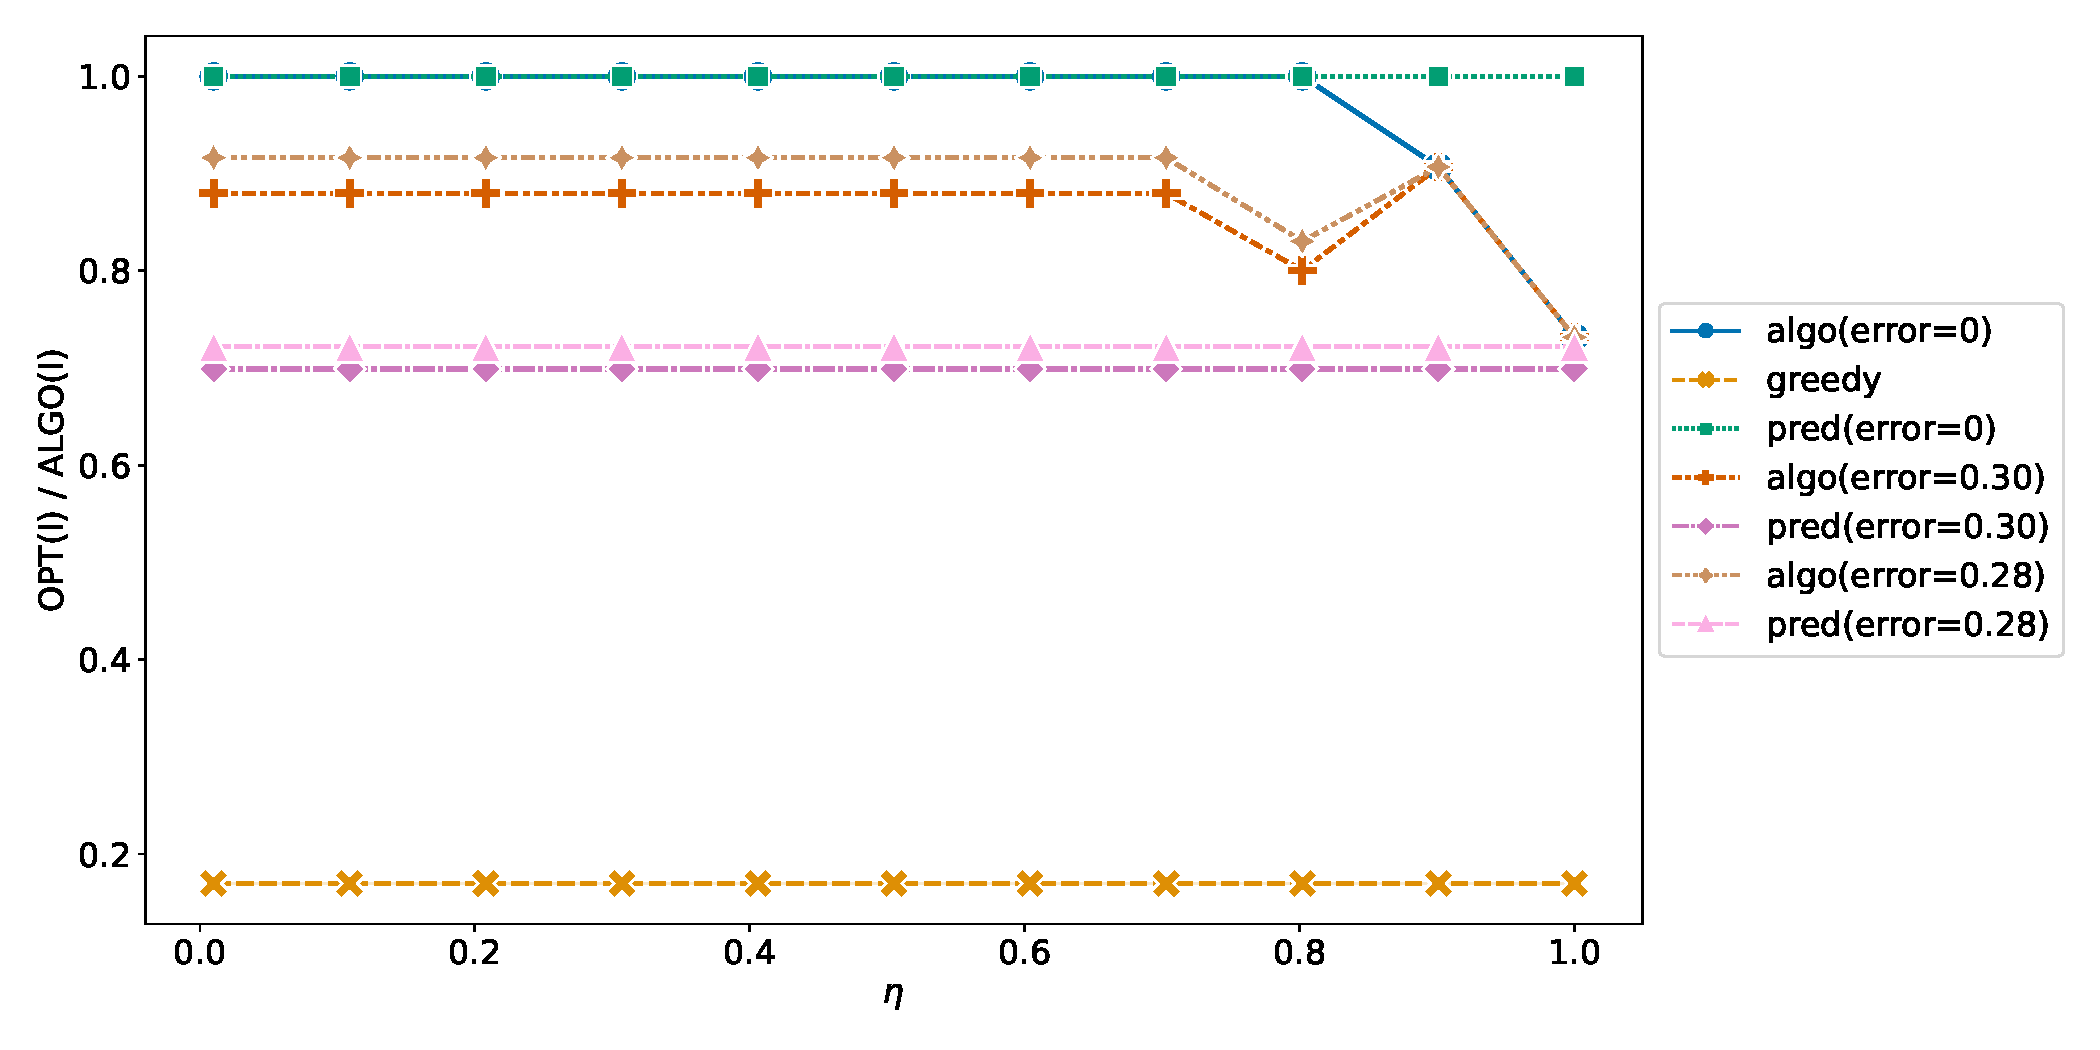
\includegraphics[width=\linewidth]{Img/figure2.pdf}
    \caption{Experiment result. The x-axis show the confidence in the prediction, where 0 means higher confidence. The y-axis show the competitive ratio compared to the optimal offline integral solution. The different colors (also markers) show the result of the algorithm with different prediction error rates and the solutions of the greedy algorithm and the prediction alone. The input graph has $20$ vertices, $69$ arcs, and $10$ requests.}
    \label{fig:experiment-2}
\end{figure}

\begin{figure}[!ht]
    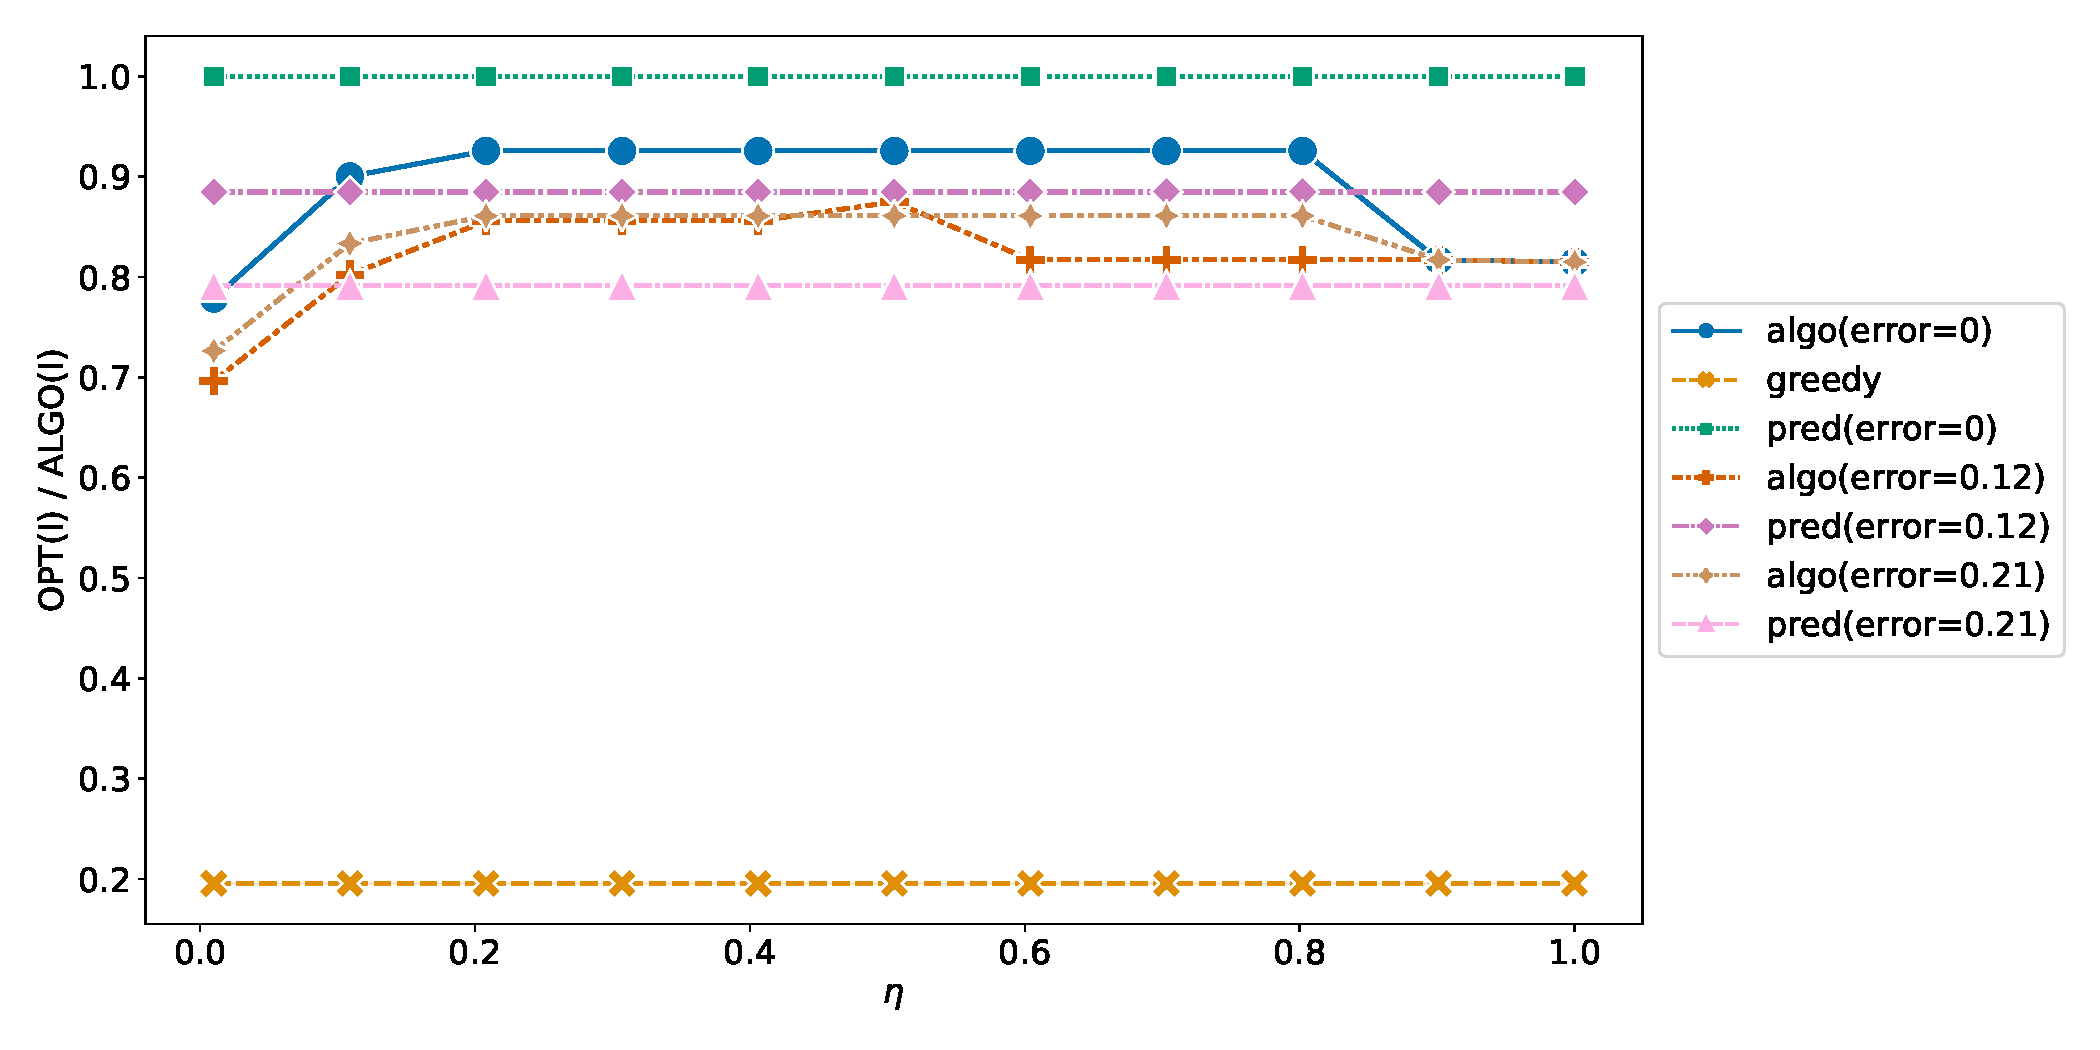
\includegraphics[width=\linewidth]{Img/figure3.pdf}
    \caption{Experiment result. The x-axis show the confidence in the prediction, where 0 means higher confidence. The y-axis show the competitive ratio compared to the optimal offline integral solution. The different colors (also markers) show the result of the algorithm with different prediction error rates and the solutions of the greedy algorithm and the prediction alone. The input graph has $30$ vertices, $73$ arcs, and $20$ requests.}
    \label{fig:experiment-3}
\end{figure}

%!TEX root = ./main.tex

\section{Counter example for the performance of the algorithm of \cite{AnandGe22:Online-Algorithms}}
\label{sec:counter-example}


Anand, Ge, Kumar and Panigrahi \cite{AnandGe22:Online-Algorithms} recently proposed online algorithms for online covering problems with multiple expert solutions.
We show here a counter example that contradicts Theorem~$2.1$ presented in Section~$3$ of their paper.
In the proof of Theorem~$2.1$ the authors state that \textit{the total cost of the algorithm is at most $3$ times the potential $\phi$ at the beginning, i.e., at most $O(\log~K)$ times the \texttt{DYNAMIC} benchmark}. However, in our counter example the total cost of their algorithm is $O(L \log(K))$ times the \texttt{DYNAMIC} benchmark, where $L$ is an arbitrary large number.

\subsection{Setting}

Algorithm $1$ (from \cite{AnandGe22:Online-Algorithms}) receives solutions from $K$ experts. The authors denote with $x_i(j,s)$ the solution from expert $s$ for variable $i$ on constraint $j$. They assume that the expert solutions are tight, formally:
%
\[ \sum_{i=1}^{n} a_{ij}\ x_{i}(j, s) = 1 \ \ \ \ \forall\ s \in [K]\]
%
The algorithm's performance is compared to the \texttt{DYNAMIC} benchmark, which is the minimum cost solution that is supported by at least one expert at each step, formally:
%
\[\texttt{DYNAMIC} = \min_{\hat{\textbf{x}} \in \hat{X}} \sum_{i=1}^{n} c_i \hat{x}_i \textnormal{, where}\]
%
\[\hat{X} = \{\hat{\textbf{x}} : \forall\ i \in [n],\ \forall\ j \in [m],\ \exists\ s \in [K] \textnormal{ where the solution } x_i(j,s) \le \hat{x}_i \}\]
%
While a constraint is not satisfied, their algorithm updates each variable with an increasing rate of
%
\[\frac{dx_i}{dt} = \frac{a_{ij}}{c_i}(x_i + \delta_{ij})\]
%
where $\delta_{ij} = \frac{1}{K} \sum_{s=1}^{K} x_i(j,s)$ is the average of the experts' solutions for $x_i$ at the arrival of constraint $j$.
Algorithm 1 of \cite{AnandGe22:Online-Algorithms} scales down the problem with $0.5$, so it does not increase any variable above $0.5$ and satisfies each constraint with value $0.5$. The exact solution is obtained by doubling the variables at the end of the execution. (This descaling is an important aspect in the authors' proof.)

\subsection{Counter example}

In the following example we reveal in an online manner a linear program parametrized by $L$ with $K$ experts and observe the behavior of Algorithm $1$ (from \cite{AnandGe22:Online-Algorithms}). This example is an extension of the pathological input for the multiplicative weight update algorithm.

\medskip

\noindent \textbf{Objective}. The example has $(L \cdot K + 1)$ variables with uniform cost:
\[ \min\ x_1 + x_2 + \dots + x_{K} + \dots + x_{2K} + \dots + x_{LK} + x_{LK+1}\]

\noindent \textbf{Constraints}. There are $L$ batches of $(K - 1)$ constraints. The first constraint of each batch has $(K+1)$ variables. The last variable ($x_{LK+1}$) is present in every constraint in every batch, but none of the experts suggests to use this variable. Within a batch, each consecutive constraint has one less variable. The experts set each variable that appears in later batches to $0$. The first batch:
%
\begin{align*}
     & \ \ \ \ x_{1} + x_{2} + \dots + x_{(K-1)} + x_{K} + x_{LK+1} \ge 1\\
\textnormal{Expert}_{1}: & \hspace{0.5cm} 1 \hspace{0.6cm} 0 \hspace{0.42cm} \dots \hspace{0.53cm} 0  \hspace{1.23cm} 0 \hspace{0.8cm} 0 \\
\textnormal{Expert}_{2}: & \hspace{0.5cm} 0 \hspace{0.6cm} 1 \hspace{0.42cm} \dots \hspace{0.53cm} 0  \hspace{1.23cm} 0 \hspace{0.8cm} 0 \\
     \vdots  & \\
\textnormal{Expert}_{K-1}: & \hspace{0.5cm} 0 \hspace{0.6cm} 0 \hspace{0.42cm} \dots \hspace{0.53cm} 1  \hspace{1.23cm} 0 \hspace{0.8cm} 0 \\
\textnormal{Expert}_{K}: & \hspace{0.5cm} 0 \hspace{0.6cm} 0 \hspace{0.42cm} \dots \hspace{0.53cm} 0  \hspace{1.23cm} 1 \hspace{0.8cm} 0 \\
     & \hspace{1.15cm} x_{2} + \dots + x_{(K-1)} + x_{K} + x_{LK+1} \ge 1\\
\textnormal{Expert}_{1}: & \hspace{0.5cm} 1 \hspace{0.6cm} 1 \hspace{0.42cm} \dots \hspace{0.53cm} 0  \hspace{1.23cm} 0 \hspace{0.8cm} 0 \\
\textnormal{Expert}_{2}: & \hspace{0.5cm} 0 \hspace{0.6cm} 1 \hspace{0.42cm} \dots \hspace{0.53cm} 0  \hspace{1.23cm} 0 \hspace{0.8cm} 0 \\
     \vdots  & \\
\textnormal{Expert}_{K-1}: & \hspace{0.5cm} 0 \hspace{0.6cm} 0 \hspace{0.42cm} \dots \hspace{0.53cm} 1  \hspace{1.23cm} 0 \hspace{0.8cm} 0 \\
\textnormal{Expert}_{K}: & \hspace{0.5cm} 0 \hspace{0.6cm} 0 \hspace{0.42cm} \dots \hspace{0.53cm} 0  \hspace{1.23cm} 1 \hspace{0.8cm} 0 \\
     \vdots  & \\
     & \hspace{2.7cm} x_{(K-1)} + x_{K} + x_{LK+1} \ge 1\\
\textnormal{Expert}_{1}: & \hspace{0.5cm} 1 \hspace{0.6cm} 1 \hspace{0.42cm} \dots \hspace{0.53cm} 1  \hspace{1.23cm} 0 \hspace{0.8cm} 0 \\
\textnormal{Expert}_{2}: & \hspace{0.5cm} 0 \hspace{0.6cm} 1 \hspace{0.42cm} \dots \hspace{0.53cm} 1  \hspace{1.23cm} 0 \hspace{0.8cm} 0 \\
     \vdots  & \\
\textnormal{Expert}_{K-1}: & \hspace{0.5cm} 0 \hspace{0.6cm} 0 \hspace{0.42cm} \dots \hspace{0.53cm} 1  \hspace{1.23cm} 0 \hspace{0.8cm} 0 \\
\textnormal{Expert}_{K}: & \hspace{0.5cm} 0 \hspace{0.6cm} 0 \hspace{0.42cm} \dots \hspace{0.53cm} 0  \hspace{1.23cm} 1 \hspace{0.8cm} 0 \\
\end{align*}

During the first constraint of every batch, the experts' solutions form an identity matrix. With each disappearing variable in the consecutive constraints, experts who suggested to use variables which are no longer available, choose to set the variable with the smallest index. Consequently, $(K-1)$ experts suggest to use variable $x_{(K-1)}$ and one expert suggests to use $x_K$ during the last constraint in the first batch. The pattern of the experts' solutions are identical for each batch. The constraints of the $l^{th}$ batch ($ 1 \le l \le L)$ are:
%
\begin{align*}
     x_{(l-1) K + 1} + x_{(l-1) K + 2} + \dots + x_{(l-1) K + (K-1)} + x_{lK} + x_{LK+1} \ge & \ 1\\
     x_{(l-1) K + 2} + \dots + x_{(l-1) K + (K-1)} + x_{lK} + x_{LK+1} \ge & \ 1\\
     \vdots &\\
     x_{(l-1) K + (K-1)} + x_{lK} + x_{LK+1} \ge & \ 1\\
\end{align*}
%

\begin{claim}
The objective value of Algorithm $1$ (from \cite{AnandGe22:Online-Algorithms}) on our example is $O(L \log(K))$ times the \texttt{DYNAMIC} benchmark.
\end{claim}
%
\begin{proof}
The optimal solution $\vect{x}^{*}$ of the \texttt{DYNAMIC} benchmark is the solution in which $x^{*}_{LK+1} = 1$ and $x^{*}_{i} = 0$ for $i \neq LK + 1$.
We verify that $\vect{x}^{*} \in \hat{X}$. For each $i \neq l K$ where $1 \leq l \leq L$, and for each constraint $m$, $x^{*}_{i} \geq 0 = x_{i}(m,K)$.
For $i = l K$, and for each constraint $m$, $x^{*}_{i} \geq 0 = x_{i}(m,1) = x_{i}(m,2) = \ldots = x_{i}(m,K-1)$.
Moreover, $\vect{x}^{*}$ satisfies all constraints (since variable $x_{LK+1}$ appears in all constraints).
Hence, $\vect{x}^{*} \in \hat{X}$. Subsequently, the objective value of the \texttt{DYNAMIC} benchmark is $1$.

     By the design of Algorithm $1$, the increasing rate of $x_{LK+1}$ is zero throughout the execution, and the variables which are not part of the current constraint are not increased. During the first constraint of each batch, the increasing rate of the first $K$ variables in the batch is $1/K$, since the increasing rate of variable $x_i$ is $(x_i + \frac{1}{K} \sum_{s=1}^{K} x_i(1,s))$ and initially every variable is set to zero. At the second constraint, the increasing rate of the second variable in the batch is higher than the other variables' increasing rate, because the first expert also uses this variable in its solution. Therefore, the increasing rate of the second variable is $(x_{(l-1) K + 2} + 2/K)$, while the other remaining expert variables in the constraint have an increasing rate of $(x_i + 1/K)$. Following the same reasoning (apart from the first constraint in the batch), the variable with the smallest index in the constraint has a higher increasing rate, than the other variables. During the last constraint of each batch, the increasing rate of the last two remaining expert variables are
     $(x_{(l-1) K + (K-1)} + (K-1)/K)$ and $(x_{lK} + 1/K)$. Keeping the increasing rates and the constraint satisfaction in mind, we can lower bound the value of each variable:
     %
     \begin{align*}
          \frac{1}{K} \ \le& \ x_{(l-1) K + 1} \\
          \frac{1}{K-1} \ \le& \ x_{(l-1) K + 2} \\
          \frac{1}{K-2} \ \le& \ x_{(l-1) K + 3} \\
          & \ \vdots \\
          \frac{1}{3} \ \le& \ x_{(l-1) K + (K-2)} \\
          \frac{1}{2} \ \le& \ x_{(l-1) K + (K-1)} \\
          \frac{1}{K} \ \le& \ x_{lK} \\
     \end{align*}

     Summing the terms together, we get that the objective value increases at least with $O(\log K)$ during each batch. There are $L$ batches, so the total cost of Algorithm $1$ is at least $O(L \log(K))$,
     while the total cost of the \texttt{DYNAMIC} benchmark is $1$, which concludes the proof.
\end{proof}

\subsection{Comparison}

In this specific counter-example, the \texttt{LIN-COMB} benchmark is equivalent to the static best-expert benchmark, i.e., the solution of Expert$_K$. The objective value of \texttt{LIN-COMB} is $L$ (since the optimal solution sets $x_{lK}$ variables for $1 \leq l \leq L$  to 1 and other variables to 0). In this counter-example, the objective value of our algorithm is $O(L\log K)$. Consequently, our proposed algorithm is $O(\log K)$ competitive in the \texttt{LIN-COMB} benchmark.

%!TEX root = ./main.tex

\section{Online \emph{linear} covering with experts}

\subsection{Performance Analysis}
As $w^{t}$ is the optimal solution of the convex program and ($\gamma^t,\ \lambda_{i},\ \mu_{i}^{t}$) is the optimal solution of its dual, the following Karush-Kuhn-Tucker (KKT) and complementary slackness conditions hold.

\begin{align*}
   \biggl[ \sum_{i=1}^{n} a_{i}^{t} \biggl( \sum_{k=1}^{K}  \hat{s}_{i,k}^{t} w_{i,k}^{t} \biggr) - 1 \biggr] \gamma^{t} &= 0 \qquad \forall\ t \\
   \biggl[ \sum_{k=1}^{K}  w_{i,k}^{t}  - 1 \biggr] \lambda_{i} &= 0 \qquad \forall\ i, t \\
   \biggl[ \sum_{k=1}^{K}  s_{i,k}^{t} w_{i,k}^{t} \biggr] \mu_{i}^{t} &= 0 \qquad \forall\ i, t \\
%
 c_{i} s_{i,k}^{t} \ln \left( \frac{\sum_{k=1}^{K} s_{i,k}^{t} w_{i,k}^{t} + \delta_{i}^{t}}{\sum_{k=1}^{K}  s_{i,k}^{t-1}w_{i,k}^{t-1}  + \delta_{i}^{t-1}} \right)
    	- a_{i}^{t} \hat{s}_{i,k}^{t} \gamma^{t} - \lambda_{i} - s_{i,k}^{t} \mu_{i}^{t} &= 0	\qquad \forall\ i,k,t \\
	%
	\gamma^{t}, \lambda_{i}, \mu_{i}^{t} &\geq 0 \qquad \forall\ i, t
\end{align*}

Moreover, if $\sum_{k} w_{i,k}^{t} s_{i,k}^{t} > 0$, meaning that $\mu_{i}^{t} = 0$, then
\begin{align}	\label{eq:KKT1}
   c_{i} s_{i,k}^{t} \ln \left( \frac{\sum_{k=1}^{K} s_{i,k}^{t} w_{i,k}^{t}  + \delta_{i}^{t}}{\sum_{k=1}^{K}  s_{i,k}^{t-1}w_{i,k}^{t-1}  + \delta_{i}^{t-1}} \right)
    	- a_{i}^{t} \hat{s}_{i,k}^{t} \gamma^{t} - \lambda_{i} = 0
\end{align}

\paragraph{Dual variables and feasibility.} We set the dual variables of the linear program relaxation of our \texttt{LIN-COMB} benchmark based on the dual variables of the convex program used inside the algorithm. The dual formulation is visible on \cref{fig:relaxation}.
%
\begin{align*}
    \alpha^{t} &= \frac{1}{\ln(K\rho)}  \biggl( \gamma^{t} + \sum_{i=1}^{n} \lambda_{i} \biggr), \\
    \beta_{i}^{t} &= \frac{1}{\ln(K\rho)} c_i \ln \left(\frac{ (1 + 1/K) \cdot \max_{t'} \sum_{k=1}^{K} s_{i,k}^{t'}}{\sum_{k=1}^{K}  s_{i,k}^{t-1} w_{i,k}^{t-1} + \delta_{i}^{t-1}}\right)
\end{align*}
%
where recall that $\rho = \max_{i, t',t''} \left\{\frac{\sum_{k=1}^{K} s_{i,k}^{t'}}{\sum_{k=1}^{K} s_{i,k}^{t''}} : \sum_{k=1}^{K} s_{i,k}^{t''} > 0 \right\}$.

\begin{lemma} \label{lem:covering-feasibility}
The $x_{i}^{t}$ solutions set by the algorithm for the original covering problem and the dual variables $(\alpha^{t}, \beta_{i}^{t})$ of the \texttt{LIN-COMB} benchmark's linear program relaxation are feasible.
\end{lemma}
%
\begin{proof}
We first prove that the $x_{i}^{t}$ variables satisfy the covering constraints by induction. At time 0, no constraint has been released yet, and every variable is set to 0. This all-zero solution is feasible. Let us assume that the algorithm provides feasible solutions up to time $t-1$. At time $t$, the algorithm maintains the inequality $x_{i}^{t} \geq x_{i}^{t-1}$, so all constraints $t'$ where $t' < t$ are satisfied. Besides, $x_{i}^{t}$ is always at least
$\sum_{k} w_{i,k}^{t} s_{i,k}^{t}$, which is larger than $\sum_{k} w_{i,k}^{t} \hat{s}_{i,k}^{t}$ since $s_{i,k}^{t} \geq \hat{s}_{i,k}^{t}$
for all $i,k$ due to the preprocessing step. Hence, the constraint $t$ is also satisfied. Formally,
$$
\sum_{i=1}^{n} a_{i}^{t} x_{i}^{t}  \geq \sum_{i=1}^{n} a_{i}^{t} \biggl( \sum_{k=1}^{K} w_{i,k}^{t}  \hat{s}_{i,k}^{t} \biggr) \geq 1.
$$

In the remaining part of the proof, we show the feasibility of $\alpha^{t}$ and every $\beta_{i}^{t}$.
Since $ \gamma^{t} \geq 0$ and $\lambda_{i} \geq 0$ for all $i$ and $t$, we get that $\alpha^{t} \geq 0$.
When we set $\beta_{i}^{t}$, the nominator of the logarithm term is always larger than the denominator, and it is smaller than $(K\rho)$-times the denominator. Consequently, $0 \leq \beta_{i}^{t} \leq c_{i}$. Furthermore,
%
\begin{align*}
    \beta_{i}^{t+1} - \beta_{i}^{t}
    	&= - \frac{1}{\ln(K\rho)} c_i \ln \left( \frac{\sum_{k=1}^{K}  s_{i,k}^{t} w_{i,k}^{t} + \delta_{i}^{t}}{\sum_{k=1}^{K}  s_{i,k}^{t-1}w_{i,k}^{t-1} + \delta_{i}^{t-1}} \right).
\end{align*}
%
Since $\sum_{i} a_{i}^{t} \hat{s}_{i,k}^{t} = 1$, using the KKT conditions, we get:
\begin{align*}
\alpha^{t} + \sum_{i=1}^{n} s_{ik}^{t} \left(\beta_{i}^{t+1} - \beta_{i}^{t}\right)
&= \frac{1}{\ln(K\rho)} \biggl( \gamma^{t} + \sum_{i=1}^{n} \lambda_{i} \biggr)
	- \frac{1}{\ln(K\rho)}  \sum_{i=1}^{n} s_{i,k}^{t} c_i \ln \left( \frac{\sum_{k=1}^{K}  s_{i,k}^{t} w_{i,k}^{t} + \delta_{i}^{t}}{\sum_{k=1}^{K}  s_{i,k}^{t-1}w_{i,k}^{t-1} + \delta_{i}^{t-1}} \right) \\
%
&= \frac{1}{\ln(K\rho)} \biggl[ \gamma^{t} + \sum_{i=1}^{n} \lambda_{i} - \sum_{i=1}^{n} \left( a_{i}^{t} \hat{s}_{i,k}^{t} \gamma^{t} + \lambda_{i} + s_{i,k}^{t} \mu_{i}^{t} \right) \biggr] \\
%
&\leq 0
\end{align*}
\end{proof}

\begin{theorem} \label{covering-theorem-proof}
The algorithm is $O(\ln(K \rho))$-competitive with the \texttt{LIN-COMB} benchmark.
\end{theorem}
%
\begin{proof} \cref{lem:covering-feasibility} proved that our algorithm creates feasible solutions for the dual problem of the \texttt{LIN-COMB} benchmark's relaxation and for the original covering problem. We show that the algorithm's solution increases the primal objective value of the original covering problem by at most $O(\ln(K \rho))$ times the value of the relaxation's dual solution, which serves as the lower bound on the \texttt{LIN-COMB} benchmark (the best linear combination of the experts' solutions).
\begin{align}
	 \sum_{i=1}^{n} &c_{i} (x_{i}^{t} - x_{i}^{t-1})
		= \sum_{i: x_{i}^{t} > x_{i}^{t-1}} c_{i}(x_{i}^{t} - x_{i}^{t-1}) &&  \notag \\
		%
		&\leq \sum_{i: x_{i}^{t} > x_{i}^{t-1}} c_{i}(x_{i}^{t} + \delta_{i}^{t}) \ln \left(\frac{x_{i}^{t} + \delta_{i}^{t}}{x_{i}^{t-1} + \delta_{i}^{t}}\right) \\
		%
		&\leq \sum_{i: x_{i}^{t} > x_{i}^{t-1}} c_{i} (x_{i}^{t} + \delta_{i}^{t}) \ln \left(\frac{x_{i}^{t} + \delta_{i}^{t}}{x_{i}^{t-1} + \delta_{i}^{t-1}}\right) \\
		%
		&= \sum_{i: x_{i}^{t} > x_{i}^{t-1}} c_{i} \left[ \left(\sum_{k=1}^{K}  s_{i,k}^{t} w_{i,k}^{t} + \frac{1}{K} \sum_{k=1}^{K} s_{i,k}^{t} \right)
			\ln \left(\frac{ \sum_{k=1}^{K}  s_{i,k}^{t} w_{i,k}^{t} + \delta_{i}^{t}}{x_{i}^{t-1} + \delta_{i}^{t-1}}  \right) \right] \\
%
&\leq \sum_{i: x_{i}^{t} > x_{i}^{t-1}} c_{i} \left[ \left(\sum_{k=1}^{K}  s_{i,k}^{t} w_{i,k}^{t} + \frac{1}{K} \sum_{k=1}^{K} s_{i,k}^{t} \right)
			\ln \left(\frac{ \sum_{k=1}^{K}  s_{i,k}^{t} w_{i,k}^{t} + \delta_{i}^{t}}{\sum_{k=1}^{K}  s_{i,k}^{t-1} w_{i,k}^{t-1} + \delta_{i}^{t-1}}  \right) \right]\\
%
	&= \sum_{i: x_{i}^{t} > x_{i}^{t-1}} \sum_{k=1}^{K} (w_{i,k}^{t} + 1/K) c_{i} s_{i,k}^{t}
				\ln \left(\frac{ \sum_{k=1}^{K} s_{i,k}^{t} w_{i,k}^{t}  + \delta_{i}^{t}}{\sum_{k=1}^{K}  s_{i,k}^{t-1} w_{i,k}^{t-1}  + \delta_{i}^{t-1}}  \right) \notag \\
%
%\end{align}
%%
%\begin{align}
%
&=  \sum_{i: x_{i}^{t} > x_{i}^{t-1}} \sum_{k=1}^{K} (w_{i,k}^{t} + 1/K) \biggl( a_{i}^{t} \hat{s}_{i,k}^{t} \gamma^t + \lambda_{i} \biggr) \\
%
%
&\leq \sum_{i=1}^{n} \sum_{k=1}^{K} (w_{i,k}^{t} + 1/K) \biggl( a_{i}^{t} \hat{s}_{i,k}^{t} \gamma^t + \lambda_{i} \biggr) \notag \\
%
&= \sum_{i=1}^{n} a_{i}^{t} \biggl(\sum_{k=1}^{K} w_{i,k}^{t} \hat{s}_{i,k}^{t} \biggr) \gamma^t + \sum_{i=1}^{n} \biggl( \sum_{k=1}^{K} w_{i,k}^{t} \biggr) \lambda_{i}
+ \frac{1}{K}  \sum_{k=1}^{K} \biggl( \sum_{i=1}^{n} a_{i}^{t}  \hat{s}_{i,k}^{t}  \biggr) \gamma^t + \frac{1}{K} \sum_{k=1}^{K} \sum_{i=1}^{n} \lambda_{i} 		\notag \\
%
&= 2 \gamma^{t} + 2\sum_{i=1}^{n} \lambda_{i} = 2\ln(K \rho) \alpha^{t}
\end{align}
%
The above corresponding transformations hold since:
\begin{compactenum}[(1)]
	\setcounter{enumi}{1}
	\item follows from the inequality $a - b \leq a \ln(a/b)$ for all $0 < b \leq a$;
	\item holds since $\delta_{i}^{t} \geq \delta_{i}^{t-1}$ (because $s_{i,k}^{t} \geq s_{i,k}^{t-1}$ for all $i,k,t$);
	\item is valid because $x_{i}^{t} > x_{i}^{t-1}$, so $x_{i}^{t} = \sum_{k}  s_{i,k}^{t} w_{i,k}^{t}$;
	\item is by the design of the algorithm: $x_{i}^{t-1} \geq \sum_{k}  s_{i,k}^{t-1} w_{i,k}^{t-1}$;
	\setcounter{enumi}{5}
	\item since given that $x_{i}^{t} > x_{i}^{t-1} \geq 0$
	(so $\sum_{k}  s_{i,k}^{t} w_{i,k}^{t} = x_{i}^{t} > 0$), the KKT condition (\ref{eq:KKT1}) applies;
	\item is true due to the complementary slackness conditions
		and that $\sum_{i} a_{i}^{t}  \hat{s}_{i,k}^{t} = 1$.
\end{compactenum}
\end{proof}

%!TEX root = ./main.tex

\section{Online \emph{convex} covering with experts} \label{sec:convex}

\subsection{Benchmark reformulation for the algorithm}

While linear programs are suitable to represent many optimization problems, they are not expressive enough to capture some practically relevant problems (for example, makespan minimization and congestion management). This section takes a step further towards a general framework and proposes an algorithm with multiple experts for $0$-$1$ optimization problems with convex objectives and linear constraints.

The performance guarantee proof of our previous algorithm relies on the primal-dual method, which bounds the algorithm's total cost by bounding at each time step the primal with the dual increase.
The \texttt{LIN-COMB} benchmark's convex objective function (visible on \cref{fig:benchmark}) does not allow us to express the objective's cost by additive terms like in the linear case. To keep the primal-dual proving technique, we reformulate the \texttt{LIN-COMB} benchmark as finding the minimum cost linear combination among all possible linear combinations. This formulation has an exponential number of variables and constraints, but it transforms the convex objective function into a linear one.

To explain the reformulation, let us first define $\mathcal{E} = \{1,2,\dots,n\}$ as a set that contains all the indices of the original covering problem's variable $x$. Then, let $S \subseteq \mathcal{E}$ be a solution, if $\vect{1}_{S}$ corresponds to a feasible solution. Recall that we consider $0$-$1$ optimization problems, so each coordinate $x_i$ of a feasible solution has a value at most $1$. Let $z_{S}$ be a (relaxed) indicator variable for solution $S$. If $z_{S} = a$, for some $a \in (0,1]$, then every variable $x_{i} = a$ if $i \in S$, and $x_{i} = 0$ if $i \notin S$. Otherwise, $z_S = 0$. In other words, $z_{S}$ indicates the fraction with which the solution $S$ participates in the final solution. The new formulation is visible on \cref{fig:reformulation} and its dual on \cref{fig:ref-dual}. Intuitively, $y_S^{t}$ indicates the fractional increase of the usage of solution $S$ at time $t$. The second constraint guarantees that if the linear combination of the experts' solutions sets a variable $x_i$ to a non-zero value, then every solution that includes $x_i$, must be used as well. The third constrain guarantees that we have a linear combination of the feasible solutions.

\begin{figure}[ht]
    \begin{mdframed}
        \vspace{-8pt}
        \begin{align*}
            && \min \sum_{t = 1}^{T} \sum_{S} & c_S y_S^t \\
            %
            (\alpha^{t}) \qquad && \sum_{k=1}^{K} w_{k}^{t} & \geq 1  & \forall\ t \\
            %
            (\beta_{i}^{t}) \qquad && \sum_{S: i \in S} z_{S}^{t} &\ge \sum_{k=1}^{K} s_{i,k}^{t} w_{k}^{t}   &\forall\ i,t\\
            %
            (\gamma^{t}) \qquad && \sum_{S} z_{S}^{t} &= 1   &\forall\ t\\
            %
            (\xi_{S}^{t}) \qquad && y_{S}^{t} &= z_{S}^{t} - z_{S}^{t-1}   &\forall\ S,t\\
            %
            && w_{k}^{t}, y_{S}^{t}, z_{S}^{t} & \ge 0 & \forall\ k,S,t
        \end{align*}
    \end{mdframed}
    \caption{Reformulation and relaxation of the \texttt{LIN-COMB} benchmark}
    \label{fig:reformulation}
\end{figure}

The new formulation of the \texttt{LIN-COMB} benchmark lower bounds its original formulation. According to the theorem of weak duality, the dual of the new formulation is a lower bound to the new formulation. Our proposed algorithm sets the variable $x$ of the original covering problem and the dual of the new formulation of the \texttt{LIN-COMB} benchmark. Afterwards, we show that at every time step, the increase of the objective cost in the original covering problem is bounded by the increase of the dual objective cost of the \texttt{LIN-COMB} benchmark's reformulation.

\clearpage

\begin{figure}[ht]
    \begin{mdframed}
        \vspace{-8pt}
        \begin{align*}
            && \max \sum_{t=1}^{T}  (\alpha^{t} &+ \gamma^{t}) \\
        %
            (w_{k}^{t}) \qquad && \alpha^{t} - \sum_{i=1}^{n} s_{i,k}^{t} \beta_{i}^{t} &\leq 0  &\forall\ k,t\\
        %
            (y_{S}^{t}) \qquad && \xi_{S}^{t}   &\leq c_{S}  &\forall\ S,t \\
        %
            (z_{S}^{t}) \qquad && \sum_{i \in S}\beta_{i}^{t} + \gamma^{t} - \xi_{S}^{t} + \xi_{S}^{t+1}  &\leq 0  &\forall\ S,t \\
        %
            && \alpha^{t}, \beta_{i}^{t} & \ge 0 & \forall\ S,i,t
        \end{align*}
    \end{mdframed}
    \caption{Dual formulation of the reformulation of the \texttt{LIN-COMB} benchmark}
    \label{fig:ref-dual}
\end{figure}

\subsection{Convex objective function properties} \label{sec:f-properties}

During our algorithm's description and analysis, we use the following two notions of function smoothness. We assume that the original covering problem's convex objective function $f$ is $L$ Lipschitz-smooth and $(\lambda, \mu)$-locally-smooth.

\begin{definition}[Lipschitz-smoothness]
    A function $f$ is Lipschitz-smooth with a constant $L$, if its derivatives are Lipschitz-continuous with the constant $L$. Formally, for all $x$ and $y$:
    \[\|\nabla f(x) - \nabla f(y)\| \le L \|x - y\|\]
\end{definition}

\begin{definition}[$(\lambda,\mu)$-local-smoothness\cite{Thang20:Online-Primal-Dual}]
    Let $\mathcal{E}$ be a set of $n$ resources.
    A differentiable function $F: [0,1]^{n} \rightarrow \mathbb{R}^{+}$ is $(\lambda,\mu)$-\emph{locally-smooth}
    if for every set $S \subseteq \mathcal{E}$, and for every set of $|S|$ arbitrary vectors $\vect{x}^{i} \in [0,1]^{n}$ where $i \in S$, the following inequality holds:
    \begin{equation*}	\label{eq:min-local-smooth}
    \sum_{i \in S} \nabla_{i} F(\vect{x}^{i}) \leq \lambda F\bigl( \vect{1}_{S} \bigr) + \mu F\bigl( \vect{x} \bigr)
    \end{equation*}
    where $\vect{x}$ is a vector whose every coordinate $x_{i'} = \max_{i}\{x^{i}_{i'}\}$ (formally, $\vect{x} := \bigvee_{i \in S} \vect{x}^{i}$);
    and $\nabla_{i} F(\vect{x})$ denotes $\partial F(\vect{x})/\partial x_{i}$.
\end{definition}

\subsection{Algorithm description}

\paragraph{Preprocessing.} We apply the preprocessing techniques of the previous algorithm to this algorithm as well, including the dummy expert to avoid division by zero. For details see \cref{sec:algo}.

\clearpage

\paragraph{Algorithm 2.} \label{algo-convex}

At the arrival of the $t^{\text{th}}$ constraint,
\begin{compactenum}
	\item solve the following convex program and set $w^t$ to be the obtained optimal solution

\begin{align*}
\min_{w} \biggl\{\sum_{i=1}^{n}
    \nabla_{i} & f\bigl(x^{t-1} \bigr) \biggl[  \biggl(\sum_{k=1}^{K} s_{i,k}^{t} w_{i,k}  + \delta_{i}^{t} \biggr)
                     \ln \left(\frac{ \sum_{k=1}^{K} s_{i,k}^{t} w_{i,k}  + \delta_{i}^{t} }{\sum_{k=1}^{K} s_{i,k}^{t-1} w_{i,k}^{t-1} + \delta_{i}^{t-1}}\right)
                                    - \sum_{k=1}^{K}  s_{i,k}^{t} w_{i,k} \biggr] \\
            %
            &+ \frac{L}{2}\biggl( \sum_{k=1}^{K} s_{i,k}^{t} w_{i,k}  - 2x_{i}^{t-1} - \delta_{i}^{t} \biggr) \biggl(\sum_{k=1}^{K} s_{i,k}^{t} w_{i,k} + \delta_{i}^{t} \biggr)
                \ln \left(\frac{ \sum_{k=1}^{K} s_{i,k}^{t} w_{i,k}  + \delta_{i}^{t} }{\sum_{k=1}^{K} s_{i,k}^{t-1} w_{i,k}^{t-1}  + \delta_{i}^{t-1}}\right) \\
            %
            &- \frac{L}{4} \biggl( \sum_{k=1}^{K} s_{i,k}^{t} w_{i,k}  - 2x_{i}^{t-1} - \delta_{i}^{t} \biggr)^{2}
        \biggr\}
\end{align*}
%
\noindent subject to:
%
\begin{align*}
    (\theta^{t})  && \sum_{i=1}^{n} a_{i}^{t} \biggl( \sum_{k=1}^{K}  \hat{s}_{i,k}^{t} w_{i,k} \biggr) &\geq 1 && \forall\ t\\
%
    (\chi_{i}) && \sum_{k=1}^{K}  w_{i,k} &\geq 1 && \forall\ i\\
%
    (\nu_{i}^{t}) && \sum_{k=1}^{K} s_{i,k}^{t} w_{i,k} &\geq 0 && \forall\ i,t
\end{align*}
%
where $\delta_{i}^{t} = \frac{1}{K} \sum_{k} s_{i,k}^{t}$ and $L$ is the Lipschitz-smoothness constant of $f$.
%and recall that we set $\rho = \max_{i} \max_{t',t''} \left\{\frac{\sum_{k=1}^{K} s_{i,k}^{t'}}{\sum_{k=1}^{K} s_{i,k}^{t''}} : \sum_{k=1}^{K} s_{i,k}^{t''} > 0 \right\}$.
Note that in this program, we use the auxiliary solution $\hat{s}_{i,k}^{t}$ in the first constraint. For every $i$ where $s_{i,k}^{t} = 0$ for all $k$, the term related to $i$ is not included in the objective function of the convex program.
(We can set $w_{i,k} = 0$ for all $k$ beforehand.)
	%
	\item For all $i$, if $\sum_{k} w_{i,k}^{t} s_{i,k}^{t} > x_{i}^{t-1}$ then set $x_{i}^{t} \gets \sum_{k} w_{i,k}^{t} s_{i,k}^{t}$;
otherwise set $x_{i}^{t} \gets x_{i}^{t-1}$.
\end{compactenum}


\subsection{Performance analysis}
As $w^{t}$ is the optimal solution of the convex program and ($\theta^t,\ \chi_{i},\ \nu_{i}^{t}$) is the optimal solution of its dual, the following Karush-Kuhn-Tucker (KKT) and complementary slackness conditions hold.

\begin{align*}
   \biggl[ \sum_{i=1}^{n} a_{i}^{t} \biggl( \sum_{k=1}^{K}  \hat{s}_{i,k}^{t} w_{i,k}^{t} \biggr) - 1 \biggr] \theta^{t} &= 0 \qquad \forall \ t \\
   \biggl[ \sum_{k=1}^{K}  w_{i,k}^{t}  - 1 \biggr] \chi_{i} &= 0 \qquad \forall\ i, t \\
   \biggl[ \sum_{k=1}^{K}  s_{i,k}^{t} w_{i,k}^{t} \biggr] \nu_{i}^{t} &= 0 \qquad \forall\ i, t \\
%
 s_{i,k}^{t} \biggl[  \nabla_{i} f(x^{t-1}) + L\biggl( \sum_{k=1}^{K} s_{i,k}^{t} w_{i,k}  - x_{i}^{t-1} \biggr) \biggr] \ln \left( \frac{\sum_{k=1}^{K} s_{i,k}^{t} w_{i,k}^{t} + \delta_{i}^{t}}{\sum_{k=1}^{K}  s_{i,k}^{t-1}w_{i,k}^{t-1}  + \delta_{i}^{t-1}} \right) \\
        - a_{i}^{t} \hat{s}_{i,k}^{t} \theta^{t} - \chi_{i} - s_{i,k}^{t} \nu_{i}^{t} &= 0	\qquad \forall\ i,k,t \\
    %
    \theta^{t}, \chi_{i}, \nu_{i}^{t} &\geq 0 \qquad \forall\ i, t
\end{align*}

Moreover, if $\sum_{k} w_{i,k}^{t} s_{i,k}^{t} > 0$, meaning that $\nu_{i}^{t} = 0$, then
\begin{align}	\label{eq:KKT2}
 s_{i,k}^{t} \biggl[  \nabla_{i} f(x^{t-1}) + L\biggl( \sum_{k=1}^{K} s_{i,k}^{t} w_{i,k}  - x_{i}^{t-1} \biggr) \biggr] \ln \left( \frac{\sum_{k=1}^{K} s_{i,k}^{t} w_{i,k}^{t} + \delta_{i}^{t}}{\sum_{k=1}^{K}  s_{i,k}^{t-1}w_{i,k}^{t-1}  + \delta_{i}^{t-1}} \right)
        - a_{i}^{t} \hat{s}_{i,k}^{t} \theta^{t} - \chi_{i}^{t} = 0
\end{align}

\clearpage

\paragraph{Dual variables and feasibility.} We set the dual variables of the reformulation of our \texttt{LIN-COMB} benchmark based on the dual variables of the convex program used inside the algorithm. The dual formulation is visible on \cref{fig:ref-dual}. The constants $\lambda$ and $\mu$ correspond to the $(\lambda,\mu)$-local-smoothness, and $L$ to the Lipschitz-smoothness of $f$ (see the definitions at \cref{sec:f-properties}).
%
\begin{align*}
    \alpha^{t} &= \frac{1}{\lambda}  \biggl( \theta^{t} + \sum_{i=1}^{n} \chi_{i} \biggr), \\
    %
    \beta_{i}^{t} &= \frac{1}{\lambda} \biggl[  \nabla_{i} f(x^{t-1}) + L\biggl( \sum_{k=1}^{K} s_{i,k}^{t} w_{i,k}  - x_{i}^{t-1} \biggr) \biggr] \ln \left( \frac{\sum_{k=1}^{K} s_{i,k}^{t} w_{i,k}^{t} + \delta_{i}^{t}}{\sum_{k=1}^{K}  s_{i,k}^{t-1}w_{i,k}^{t-1}  + \delta_{i}^{t-1}} \right) \\
    %
    \xi_{S}^{t} &= \frac{1}{\lambda} \sum_{i \in S} \nabla_{i} f(x^{t-1}) \ln \left( \frac{(1 + 1/K) \cdot \max_{t'} \sum_{k=1}^{K} s_{i,k}^{t'}}{\sum_{k=1}^{K}  s_{i,k}^{t-1}w_{i,k}^{t-1}  + \delta_{i}^{t-1}} \right) - \frac{\mu}{\lambda} \ln(K\rho)  f(x^{t-1})\\
    %
    \gamma^{t} &= -  \frac{1}{\lambda} \sum_{i=1}^{n} \biggl[  \nabla_{i} f(x^{t-1}) + L\biggl( \sum_{k=1}^{K} s_{i,k}^{t} w_{i,k}  - x_{i}^{t-1} \biggr) \biggr]  \ln \left( \frac{\sum_{k=1}^{K} s_{i,k}^{t} w_{i,k}^{t} + \delta_{i}^{t}}{\sum_{k=1}^{K}  s_{i,k}^{t-1}w_{i,k}^{t-1}  + \delta_{i}^{t-1}} \right) \\
        & \quad - \frac{1}{\lambda} \sum_{i=1}^{n} \biggl[ \nabla_{i} f(x^{t}) \ln \left( \frac{(1 + 1/K) \cdot \max_{t'} \sum_{k=1}^{K} s_{i,k}^{t'}}{\sum_{k=1}^{K}  s_{i,k}^{t}w_{i,k}^{t}  + \delta_{i}^{t}} \right) -  \nabla_{i} f(x^{t-1}) \ln \left( \frac{(1 + 1/K) \cdot \max_{t'} \sum_{k=1}^{K} s_{i,k}^{t'}}{\sum_{k=1}^{K}  s_{i,k}^{t-1}w_{i,k}^{t-1}  + \delta_{i}^{t-1}} \right) \biggr] \\
    & \quad + \frac{\mu}{\lambda} \ln(K\rho) f(x^{t}) - \frac{\mu}{\lambda} \ln(K\rho) f(x^{t-1})
\end{align*}
%
Recall that $\rho = \max_{i, t',t''} \left\{\frac{\sum_{k=1}^{K} s_{i,k}^{t'}}{\sum_{k=1}^{K} s_{i,k}^{t''}} : \sum_{k=1}^{K} s_{i,k}^{t''} > 0 \right\}$.

\begin{lemma} \label{lem:convex-covering-feasibility}
The original covering problem's $x_{i}^{t}$ solution set by the algorithm and the dual variables $(\alpha^{t}, \beta_{i}^{t}, \xi_S^t, \gamma^t)$ of the reformulated \texttt{LIN-COMB} benchmark are feasible up to a factor of $\ln (K\rho)$.
\end{lemma}
%
\begin{proof}
We first prove that the $x_{i}^{t}$ variables satisfy the covering constraints by induction. At time~0, no constraint has been released yet, and every variable is set to 0. This all-zero solution is feasible. Let us assume that the algorithm provides feasible solutions up to time $t-1$. At time~$t$, the algorithm maintains the inequality $x_{i}^{t} \geq x_{i}^{t-1}$, so all constraints $t'$ where $t' < t$ are satisfied. Besides, $x_{i}^{t}$ is always at least
$\sum_{k} w_{i,k}^{t} s_{i,k}^{t}$, which is larger than $\sum_{k} w_{i,k}^{t} \hat{s}_{i,k}^{t}$ since $s_{i,k}^{t} \geq \hat{s}_{i,k}^{t}$
for all $i,k$ due to the preprocessing step. Hence, constraint $t$ is also satisfied, formally,
$$
\sum_{i=1}^{n} a_{i}^{t} x_{i}^{t}  \geq \sum_{i=1}^{n} a_{i}^{t} \biggl( \sum_{k=1}^{K} \hat{s}_{i,k}^{t} w_{i,k}^{t} \biggr) \geq 1.
$$

In the remaining part of the proof, we show the feasibility of the dual solution. The dual constraints are visible on \cref{fig:ref-dual}.
The first constraint follows from the KKT conditions and from the fact that $\sum_{i} a_i^{t} \hat{s}_{i,k}^{t} = 1$.
The second constraint is satisfied because
%
\begin{align*}
\xi_{S}^{t} &= \frac{1}{\lambda} \sum_{i \in S} \nabla_{i} f(x^{t-1}) \ln \left( \frac{(1 + 1/K) \cdot \max_{t'} \sum_{k=1}^{K} s_{i,k}^{t'}}{\sum_{k=1}^{K}  s_{i,k}^{t-1}w_{i,k}^{t-1}  + \delta_{i}^{t-1}} \right) - \frac{\mu}{\lambda} \ln(K\rho) f(x^{t-1})  \\
&\leq \frac{1}{\lambda} \sum_{i \in S} \nabla_{i} f(x^{t-1}) \ln(K\rho)  - \frac{\mu}{\lambda} \ln(K\rho) f(x^{t-1})
\leq  \ln(K\rho) c_S
\end{align*}
%
where the last inequality holds due to the $(\lambda,\mu)$-local-smoothness. After down-scaling the variables by a factor of $\ln (K\rho)$, the second dual constraint holds.

The last constraint is satisfied due to the definition of the dual variables. We need
\begin{align*}
  \sum_{i \in S}\beta_{i}^{t} + \gamma^{t} - \xi_{S}^{t} + \xi_{S}^{t+1}  &\leq 0\\
  \sum_{i \in S}\beta_{i}^{t} - \xi_{S}^{t} + \xi_{S}^{t+1}  &\leq -\gamma^{t}
\end{align*}
%
to hold. We can simplify $\gamma^{t}$ as follows:
\begin{align*}
    \gamma^{t} &= -  \frac{1}{\lambda} \sum_{i=1}^{n} \biggl[ L\biggl( \sum_{k=1}^{K} s_{i,k}^{t} w_{i,k}  - x_{i}^{t-1} \biggr) \biggr]  \ln \left( \frac{\sum_{k=1}^{K} s_{i,k}^{t} w_{i,k}^{t} + \delta_{i}^{t}}{\sum_{k=1}^{K}  s_{ik}^{t-1}w_{i,k}^{t-1}  + \delta_{i}^{t-1}} \right) \\
    	& \quad - \frac{1}{\lambda} \sum_{i=1}^{n} \biggl[ \nabla_{i} f(x^{t}) - \nabla_{i} f(x^{t-1}) \biggr] \ln \left( \frac{(1 + 1/K) \cdot \max_{t'} \sum_{k=1}^{K} s_{i,k}^{t'}}{\sum_{k=1}^{K}  s_{ik}^{t}w_{i,k}^{t}  + \delta_{i}^{t}} \right)  \\
	& \quad + \frac{\mu}{\lambda} \ln(K\rho) f(x^{t}) - \frac{\mu}{\lambda} \ln(K\rho) f(x^{t-1})
\end{align*}
%
Now let us fix an arbitrary set $S$. Then, following the simplified form of $\gamma^t$, we have
\begin{align*}
    -\gamma^{t} &\geq     \frac{1}{\lambda} \sum_{i \in S} \biggl[ L\biggl( \sum_{k=1}^{K} s_{i,k}^{t} w_{i,k}  - x_{i}^{t-1} \biggr) \biggr]  \ln \left( \frac{\sum_{k=1}^{K} s_{i,k}^{t} w_{i,k}^{t} + \delta_{i}^{t}}{\sum_{k=1}^{K}  s_{ik}^{t-1}w_{i,k}^{t-1}  + \delta_{i}^{t-1}} \right) \\
            & \quad  \frac{1}{\lambda} \sum_{i \in S} \biggl[ \nabla_{i} f(x^{t}) - \nabla_{i} f(x^{t-1}) \biggr] \ln \left( \frac{(1 + 1/K) \cdot \max_{t'} \sum_{k=1}^{K} s_{i,k}^{t'}}{\sum_{k=1}^{K}  s_{ik}^{t}w_{i,k}^{t}  + \delta_{i}^{t}} \right)  \\
        & \quad - \frac{\mu}{\lambda} \ln(K\rho) f(x^{t}) + \frac{\mu}{\lambda} \ln(K\rho) f(x^{t-1})
\end{align*}
%
We have to show that the following is true to satisfy the third constraint:
\begin{align*}
    \sum_{i \in S}\beta_{i}^{t} - \xi_{S}^{t} + \xi_{S}^{t+1}  &\leq     \frac{1}{\lambda} \sum_{i \in S} \biggl[ L\biggl( \sum_{k=1}^{K} s_{i,k}^{t} w_{i,k}  - x_{i}^{t-1} \biggr) \biggr]  \ln \left( \frac{\sum_{k=1}^{K} s_{i,k}^{t} w_{i,k}^{t} + \delta_{i}^{t}}{\sum_{k=1}^{K}  s_{ik}^{t-1}w_{i,k}^{t-1}  + \delta_{i}^{t-1}} \right) \\
            & \quad  \frac{1}{\lambda} \sum_{i \in S} \biggl[ \nabla_{i} f(x^{t}) - \nabla_{i} f(x^{t-1}) \biggr] \ln \left( \frac{(1 + 1/K) \cdot \max_{t'} \sum_{k=1}^{K} s_{i,k}^{t'}}{\sum_{k=1}^{K}  s_{ik}^{t}w_{i,k}^{t}  + \delta_{i}^{t}} \right)  \\
            & \quad - \frac{\mu}{\lambda} \ln(K\rho) f(x^{t}) + \frac{\mu}{\lambda} \ln(K\rho) f(x^{t-1}) \\
    & = \sum_{i \in S} \frac{1}{\lambda} \biggl[  \nabla_{i} f(x^{t-1}) + L\biggl( \sum_{k=1}^{K} s_{i,k}^{t} w_{i,k}  - x_{i}^{t-1} \biggr) \biggr] \ln \left( \frac{\sum_{k=1}^{K} s_{i,k}^{t} w_{i,k}^{t} + \delta_{i}^{t}}{\sum_{k=1}^{K}  s_{i,k}^{t-1}w_{i,k}^{t-1}  + \delta_{i}^{t-1}} \right) \\
            & \quad - \frac{1}{\lambda} \sum_{i \in S} \nabla_{i} f(x^{t-1}) \ln \left( \frac{(1 + 1/K) \cdot \max_{t'} \sum_{k=1}^{K} s_{i,k}^{t'}}{\sum_{k=1}^{K}  s_{i,k}^{t-1}w_{i,k}^{t-1}  + \delta_{i}^{t-1}} \right) + \frac{\mu}{\lambda} \ln(K\rho)  f(x^{t-1}) \\
            & \quad + \frac{1}{\lambda} \sum_{i \in S} \nabla_{i} f(x^{t}) \ln \left( \frac{(1 + 1/K) \cdot \max_{t'} \sum_{k=1}^{K} s_{i,k}^{t'}}{\sum_{k=1}^{K}  s_{i,k}^{t}w_{i,k}^{t}  + \delta_{i}^{t}} \right) - \frac{\mu}{\lambda} \ln(K\rho)  f(x^{t})
\end{align*}
where the equality holds due to $\log(a/b) - \log(a/c) = \log(c/b)$.

It remains to show that $\alpha^t$ and $\beta_i^t$ are positive. Due to the KKT conditions both variables are always positive, so the lemma holds.
\end{proof}

\clearpage

\begin{theorem} \label{convex-covering-theorem}
Algorithm 2 is $O(\ln(K \rho)) \frac{\lambda}{1 - \mu \ln (K\rho)}$-competitive with the \texttt{LIN-COMB} benchmark.
\end{theorem}
%
\begin{proof} \cref{lem:convex-covering-feasibility} proved that our algorithm creates feasible solutions for the original covering problem and for the dual problem of the reformulated \texttt{LIN-COMB} benchmark. We show that the algorithm's solution increases the primal objective value of the original covering problem by at most $O(\ln(K \rho))$ times the value of the dual solution, which serves as the lower bound on the \texttt{LIN-COMB} benchmark - the best linear combination of the experts' solutions.

\begin{align}
&f(x^{t}) - f(x^{t-1}) \leq \nabla f(x^{t-1}) (x^{t} - x^{t-1}) + \frac{2L}{2} \|x^{t} - x^{t-1} \|^{2} \\
%
&\leq \sum_{i: x_{i}^{t} > x_{i}^{t-1}} \bigl[ \nabla_{i} f(x^{t-1}) + L(x_{i}^{t} - x_{i}^{t-1}) \bigr] (x_{i}^{t} - x_{i}^{t-1}) &&  \notag \\
%
&\leq \sum_{i: x_{i}^{t} > x_{i}^{t-1}} \bigl[ \nabla_{i} f(x^{t-1}) + L(x_{i}^{t} - x_{i}^{t-1}) \bigr](x_{i}^{t} + \delta_{i}^{t}) \ln \left(\frac{x_{i}^{t} + \delta_{i}^{t}}{x_{i}^{t-1} + \delta_{i}^{t}} \right) \\
%
&\leq \sum_{i: x_{i}^{t} > x_{i}^{t-1}} \bigl[ \nabla_{i} f(x^{t-1}) + L(x_{i}^{t} - x_{i}^{t-1}) \bigr] (x_{i}^{t} + \delta_{i}^{t}) \ln \left(\frac{x_{i}^{t} + \delta_{i}^{t}}{x_{i}^{t-1} + \delta_{i}^{t-1}} \right) \\
%
&= \sum_{i: x_{i}^{t} > x_{i}^{t-1}} \bigl[ \nabla_{i} f(x^{t-1}) + L(x_{i}^{t} - x_{i}^{t-1}) \bigr] \left[ \left(\sum_{k=1}^{K}  s_{i,k}^{t} w_{i,k}^{t} + \frac{1}{K} \sum_{k=1}^{K} s_{i,k}^{t} \right)
            \ln \left(\frac{ \sum_{k=1}^{K}  s_{i,k}^{t} w_{i,k}^{t} + \delta_{i}^{t}}{x_{i}^{t-1} + \delta_{i}^{t-1}}  \right) \right]\\
%
&\leq \sum_{i: x_{i}^{t} > x_{i}^{t-1}} \bigl[ \nabla_{i} f(x^{t-1}) + L(x_{i}^{t} - x_{i}^{t-1}) \bigr] \left[ \left(\sum_{k=1}^{K}  s_{i,k}^{t} w_{i,k}^{t} + \frac{1}{K} \sum_{k=1}^{K} s_{i,k}^{t} \right)
            \ln \left(\frac{ \sum_{k=1}^{K}  s_{i,k}^{t} w_{i,k}^{t} + \delta_{i}^{t}}{\sum_{k=1}^{K}  s_{i,k}^{t-1} w_{i,k}^{t-1} + \delta_{i}^{t-1}}  \right) \right]\\
%
&= \sum_{i: x_{i}^{t} > x_{i}^{t-1}} \sum_{k=1}^{K} (w_{i,k}^{t} + 1/K) s_{i,k}^{t} \bigl[ \nabla_{i} f(x^{t-1}) + L(x_{i}^{t} - x_{i}^{t-1}) \bigr]
            \ln \left(\frac{ \sum_{k=1}^{K} s_{i,k}^{t} w_{i,k}^{t}  + \delta_{i}^{t}}{\sum_{k=1}^{K}  s_{i,k}^{t-1} w_{i,k}^{t-1}  + \delta_{i}^{t-1}}  \right) \notag \\
%
&=  \sum_{i: x_{i}^{t} > x_{i}^{t-1}} \sum_{k=1}^{K} (w_{i,k}^{t} + 1/K) \biggl( a_{i}^{t} \hat{s}_{i,k}^{t} \theta^{t} + \chi_{i}^{t} \biggr)  \\
%
&\leq \sum_{i=1}^{n} \sum_{k=1}^{K} (w_{i,k}^{t} + 1/K) \biggl( a_{i}^{t} \hat{s}_{i,k}^{t} \theta^{t} + \chi_{i}^{t} \biggr) \notag \\
%
&= \sum_{i=1}^{n} a_{i}^{t} \biggl(\sum_{k=1}^{K} w_{i,k}^{t} \hat{s}_{i,k}^{t} \biggr) \theta^t + \sum_{i=1}^{n} \biggl( \sum_{k=1}^{K} w_{i,k}^{t} \biggr) \chi_{i}^{t}
+ \frac{1}{K}  \sum_{k=1}^{K} \biggl( \sum_{i=1}^{n} a_{i}^{t}  \hat{s}_{i,k}^{t}  \biggr) \theta^t + \frac{1}{K} \sum_{k=1}^{K} \sum_{i=1}^{n} \chi_{i}^{t} 		\notag \\
%
&= 2 \theta^{t} + 2\sum_{i=1}^{n} \chi_{i}^{t} \\
%
&= 2\lambda \cdot \alpha^{t}	\notag
\end{align}
%
The above corresponding transformations hold since:
\begin{compactenum}[(1)]
    \setcounter{enumi}{8}
    \item holds as $f$ is $2L$-smooth;
    \item follows from the inequality $a - b \leq a \ln(a/b)$ for all $0 < b \leq a$;
    \item holds since $\delta_{i}^{t} \geq \delta_{i}^{t-1}$ (because $s_{i,k}^{t} \geq s_{i,k}^{t-1}$ for all $i,k,t$);
    \item is valid because $x_{i}^{t} > x_{i}^{t-1}$, so $x_{i}^{t} = \sum_{k=1}^{K}  s_{i,k}^{t} w_{i,k}^{t}$;
    \item is by the design of the algorithm: $x_{i}^{t-1} \geq \sum_{k=1}^{K}  s_{i,k}^{t-1} w_{i,k}^{t-1}$;
    %\setcounter{enumi}{5}
    \item since given that $x_{i}^{t} > x_{i}^{t-1} \geq 0$
    (so $\sum_{k=1}^{K}  s_{i,k}^{t} w_{i,k}^{t} = x_{i}^{t} > 0$), the KKT condition (\ref{eq:KKT2}) applies;
    \item is true due to the complementary slackness conditions
        and that $\sum_{i=1}^{n} a_{i}^{t}  \hat{s}_{i,k}^{t} = 1$.
\end{compactenum}

\clearpage

\noindent The objective of the dual includes $\sum_{t = 1}^{T} \gamma^{t}$ as well, so it remains to bound this sum. We recall that the simplified version of $\gamma^t$ is
\begin{align*}
    \gamma^{t} &= -  \frac{1}{\lambda} \sum_{i=1}^{n} \biggl[ L\biggl( \sum_{k=1}^{K} s_{i,k}^{t} w_{i,k}  - x_{i}^{t-1} \biggr) \biggr]  \ln \left( \frac{\sum_{k=1}^{K} s_{i,k}^{t} w_{i,k}^{t} + \delta_{i}^{t}}{\sum_{k=1}^{K}  s_{ik}^{t-1}w_{i,k}^{t-1}  + \delta_{i}^{t-1}} \right) \\
    	& \quad - \frac{1}{\lambda} \sum_{i=1}^{n} \biggl[ \nabla_{i} f(x^{t}) - \nabla_{i} f(x^{t-1}) \biggr] \ln \left( \frac{(1 + 1/K) \cdot \max_{t'} \sum_{k=1}^{K} s_{i,k}^{t'}}{\sum_{k=1}^{K}  s_{ik}^{t}w_{i,k}^{t}  + \delta_{i}^{t}} \right)  \\
	& \quad + \frac{\mu}{\lambda} \ln(K\rho) f(x^{t}) - \frac{\mu}{\lambda} \ln(K\rho) f(x^{t-1})
\end{align*}
%
Since $f$ is $2L$-smooth with respect to the $\ell_{2}$-norm, we can observe that
\begin{align*}
\sum_{i=1}^{n} (\nabla_{i} f(x^{t}) -  \nabla_{i} f(x^{t-1}) \ln \left( \frac{(1 + 1/K) \cdot \max_{t'} \sum_{k=1}^{K} s_{i,k}^{t'}}{\sum_{k=1}^{K}  s_{i,k}^{t}w_{i,k}^{t}  + \delta_{i}^{t}} \right)
\leq \ln(K\rho) 2L\sqrt{n} \sum_{i=1}^{n} (x_{i}^{t} - x_{i}^{t-1})
\end{align*}
%
and after bounding the following term
%
\begin{align*}
2\biggl( \sum_{k=1}^{K} s_{i,k}^{t} w_{i,k}  - x_{i}^{t-1} \biggr) \ln \left( \frac{\sum_{k=1}^{K} s_{i,k}^{t} w_{i,k}^{t} + \delta_{i}^{t}}{\sum_{k=1}^{K}  s_{i,k}^{t-1}w_{i,k}^{t-1}  + \delta_{i}^{t-1}} \right)
\leq \ln(K\rho) (x_{i}^{t} - x_{i}^{t-1})
\end{align*}
%
we get that
\begin{align*}
\sum_{t=1}^{T} \gamma^{t} &\geq - \frac{\mu \ln (K\rho)}{\lambda} f(x^{T}) - \ln(K\rho) \frac{4L}{\lambda} \sqrt{n} \sum_{t=1}^{T} \sum_{i=1}^{n} (x_{i}^{t} - x_{i}^{t-1}) \\
&\geq - \frac{\mu \ln (K\rho)}{\lambda} f(x^{T}) - \ln(K\rho) \frac{4L}{\lambda} \sqrt{n} \sum_{i=1}^{n} x_{i}^{T}
\end{align*}
Considering both parts of the proof so far, we bound the dual objective as follows:
\begin{align*}
\sum_{t=1}^{T} (\alpha^{t} + \gamma^{t}) \geq \frac{1/2-\mu\ln (K\rho)}{\lambda} f(x^{T}) - \ln(K\rho) \frac{4L}{\lambda} \sqrt{n} \sum_{i=1}^{n} x_{i}^{T}
\end{align*}
In $0-1$ optimization, $x_{i}^{T} \leq 1$.
Hence, the theorem follows.
\end{proof}

\clearpage
%!TEX root = ./main.tex

\section{Experiments} \label{sec:exp}

In this section we include the experiments of the first algorithm for problems with a linear objective function.

\textbf{Implementation.} The first step of our first proposed algorithm is to solve a convex program. In the experiments, we approximate the optimal solution of this program using a vanilla Frank-Wolfe implementation. The linear minimization step within Frank-Wolfe is solved with the Gurobi optimizer.

\textbf{Comparison.} The best standard online algorithm for general covering problems without experts is the online multiplicative weight update (MWU) algorithm. In the experiments we compare our algorithm with the MWU algorithm. When a new constraint arrives in the online problem, the MWU algorithm increases each variable $x_i$ in the constraint with a rate of $\frac{a^t_i}{c_i}(x_i + 1/n)$, where $n$ is the total number of variables. We also compare our results with the optimum offline solution (that knows the whole instance in advance) and the average solution of the experts.
%On the following figures, we display both the first and the second layer execution results of our algorithm (see \cref{fig:my_label}).

\textbf{Input.} First, we evaluated the result of our algorithm on the pathological input of the MWU algorithm. This instance includes $n$ variables and $n$ constraints with uniform costs and coefficients. Each arriving constraint in this pathological example includes one less variable. While the optimal solution is $1$, the worst-case guarantee of MWU is $O(\log n)$. For our algorithm we provided $n$ experts, where $(n-1)$ experts suggest an adversarial trivial solution to set all variables to $1$, while $1$ expert suggests the optimal offline solution. The result of this experiment is visible on \cref{fig:exp-objective}. An important highlight: our algorithm managed to identify the good expert among the majority of adversaries, obtaining a better objective value, than MWU. Second, we experimented with the counter example (in Appendix~\ref{sec:counter-example}) which shows that the claim of \cite{AnandGe22:Online-Algorithms} is unfortunately too strong. The result is also visible on \cref{fig:exp-objective}. Finally, we generated some instances to observe the performance of our algorithm on non-specific inputs.
The specification for the instance generation includes several parameters, which we detail on \cref{fig:exp-params}. The non-specific instances try to represent instances with different 'shape', meaning that the ratio of the number of constraints and variables varies.

To further investigate the impact of the number of variables and the number of experts on our algorithm, we executed the worst case example for the MWU with several input sizes. The result is visible on \cref{fig:exp-3d}.

\textbf{Result.} Multiplicative weight update is a simple and well-performing algorithm in practice. On its pathological worst-case example, our algorithm performs better, however on most instances the expert suggestions were significantly worse than MWU, which impacted the performance of our algorithm. To some extent, our algorithm can detect the good experts and is robust against even many adversaries. We think that given a real-life problem, it is possible to construct well-performing experts (for example using past data) and with a fine-tuned convex program solver our algorithm can be of interest for various use-cases.

\begin{figure}[!ht]
\centering
\begin{tabular}{r|r|r|r|r|r|r}
          & Worst-case & Counter-ex. & & & & \\
Algo name & for MWU  & for \cite{AnandGe22:Online-Algorithms} & Inst. $1$ & Inst. $2$ & Inst. $3$ & Inst. $4$\\
\hline
OPT Offline            & 1.0 & 1.0 & 1.3 & 1.5 & 10.6 & 31.3 \\
MWU Online             & 2.9 & 2.3 & 2.0 & 1.7 & 28.1 & 63.7 \\
\hline
%Our Algo               & 1.6 & 5.8 & 24.5 & \textbf{17.5}\\
Our Algo           & {\bf 2.2} & {\bf 4.4} & {\bf 2.0} & {\bf 1.7} & {\bf 26.7}  & {\bf 61.7} \\
\hline
Avg of experts      & 9.1 & 3.5 & 16.4 & 23.3 & 1897.47 & 96.9 \\
\end{tabular}
\caption{Objective value of the experiment instances}
\label{fig:exp-objective}
\end{figure}

\begin{figure}[!ht]
\centering
\begin{tabular}{l|r|r|r|r}
Input Generation Parameters & Instance $1$ & Instance $2$ & Instance $3$ & Instance $4$ \\
\hline
Number of variables            & 10 & 10 & 44  & 30 \\
Number of constraints          & 10 & 25 & 2   & 15 \\
Min objective coefficient      & 1  & 10 & 1   & 1  \\
Max objective coefficient      & 10 & 25 & 100 & 100\\
Min constraint coefficient     & 1  & 10 & 1   & 1 \\
Max constraint coefficient     & 10 & 25 & 1   & 1 \\
Min number of zero coefficient & 0  &  1 & 11  & 5 \\
Max number of zero coefficient & 5  &  5 & 22  & 20 \\
Number of perfect experts      & 1  &  0 & 0   & 2 \\
Number of online experts       & 2  &  1 & 1   & 2 \\
Number of random experts       & 1  &  1 & 11  & 0 \\
Number of adversaries          & 1  &  1 & 0   & 0 \\
\end{tabular}
\caption{Parameters of the generated experiment instances}
\label{fig:exp-params}
\end{figure}

\begin{figure}[!ht]
    \centering
    \includegraphics[width=\linewidth]{Img/worst_case_figure.pdf}
    \caption{Experiment with varying number of variables and experts on the MWU worst-case instance}
    \label{fig:exp-3d}
\end{figure}

\end{document}
